\chapter{激光扫描共聚焦荧光寿命显微镜搭建}\label{Chap:3}

在全文的系统主线中，本章所构建的激光扫描共聚焦荧光寿命显微镜并不是与后续多光子系统相互割裂的独立平台，而是面向多光子荧光寿命成像系统构建的重要前期验证与模块化基础。一方面，共聚焦系统在扫描成像、激发与探测通道组织、多色光路切换以及同步采集链路建立等方面，与后续多光子 FLIM 系统具有高度一致的系统结构特征；另一方面，共聚焦平台具有调试灵活、信号直观、实验门槛较低等优势，适合作为多色激发架构、时序同步流程以及荧光寿命测量链路的预研平台。因此，本章通过模块化光机设计与多色快拆架构的实现，为后续多光子系统中的复杂光路组织、模式切换及寿命成像功能集成提供可迁移的工程基础。

\section{共聚焦显微镜成像原理}\label{3.1}
\subsection{宽场荧光显微镜与衍射极限}\label{3.1.1}
宽场荧光显微镜采用面照明与面探测的成像方式，即样品在整个视场范围内同时受到激发，不同空间位置产生的荧光信号也由探测器并行记录。该方式具有成像速度快、系统结构相对简单等优点，因此在生物显微成像中得到了广泛应用。然而，由于样品中焦平面以外区域同样会被激发，来自焦平面上、下方的离焦荧光也会叠加到最终图像中，从而降低图像对比度，并削弱系统的轴向分辨能力。尤其在厚样品或散射样品成像中，这一问题更加突出。

在理想衍射受限条件下，宽场显微镜的横向分辨率主要受发射波长 $\lambda_{em}$ 和物镜数值孔径 $NA$ 限制，常可用阿贝判据近似表示为:

\begin{equation}
    r=\frac{0.61\lambda_{em}}{NA}
\end{equation}

该式表明，减小工作波长或增大物镜数值孔径均有助于提高系统的横向分辨能力。然而，该表达式仅反映理想条件下的横向分辨极限，并未考虑离焦背景、像差、散射以及系统噪声等实际因素。因此，在厚样品成像中，宽场显微镜的实际成像质量通常明显低于理论极限。

从物理本质上看，显微镜的分辨能力受衍射效应约束。样品中的点光源经过高数值孔径物镜成像后，不会在像面上形成理想的几何点，而是形成具有有限尺寸的点扩散函数，其中心亮斑通常表现为艾里斑(Airy disk)。当两个发光点之间的距离小于系统 PSF 主瓣宽度时，其像强分布将发生重叠，从而无法在图像中被清晰区分。这也是传统光学显微镜受衍射极限约束的根本原因。




\subsection{激光扫描共聚焦显微镜的基本思想}\label{3.1.2}
激光扫描共聚焦显微镜(laser scanning confocal microscopy, LSCM)是在宽场荧光显微镜基础上发展起来的一种点扫描成像技术。其核心思想在于：利用高度聚焦的激发光束对样品进行逐点照明，并在探测光路的共轭像面处设置空间滤波小孔，仅允许来自焦点附近的信号有效通过，从而显著抑制离焦背景，提高图像对比度和轴向分辨能力。

``共聚焦''一词强调的是系统在光路结构上的共轭关系，即激发焦点、样品焦点以及探测小孔在光学上相互对应。具体而言，激发激光经准直和扩束后进入扫描系统，在振镜驱动下实现二维偏转；随后激光依次经过SL和TL中继，由高数值孔径物镜聚焦到样品中的某一位置，从而实现逐点扫描激发。样品产生的反射或荧光信号再经原光路返回，并通过二向色镜、分光镜等元件与激发光分离，最终在共轭像面处经小孔或光纤耦合进入探测器。

\begin{figure}[htbp]
    \centering
    \includegraphics[width=0.8\textwidth]{Fig/Fig10.pdf}
    \bicaption{激光扫描共聚焦显微镜系统原理与实现流程示意图}{Schematic of the principle and implementation workflow of a laser-scanning confocal microscope}
    \label{fig10}
\end{figure}

如图~\ref{fig10} 所示，为本文自主设计的一套LSCM系统。系统左侧配置了多种激发光源，包括 532\,nm 皮秒激光光源和白光超连续谱光源。激发光经功率调节后，通过二向色镜组进入扫描通道，在振镜驱动下完成二维扫描，再依次经过扫描透镜、管透镜和显微物镜后聚焦到载物台上的样品表面。样品产生的反射信号与荧光信号沿原光路返回，经二向色镜和偏振分光元件与激发光分离后，被透镜耦合进入探测光纤和探测器。由于探测光纤或共轭小孔仅允许来自焦点附近的信号高效通过，因此离焦背景能够得到显著抑制。

在系统控制与数据采集方面，探测器输出的模拟电信号首先进入采集卡，通过模数转换器(Analog-to-Digital Converter, ADC)完成模数转换(Analog-to-Digital, AD)，并将数字化后的信号传输至上位机，用于后续成像重建与数据分析。同时，现场可编程门阵列(Field Programmable Gate Array, FPGA)根据系统扫描参数生成控制时序，并通过数模转换器(Digital-to-Analog Converter, DAC)完成数模转换(Digital-to-Analog, DA)，输出模拟控制电压以驱动振镜控制模块，从而实现对扫描速度、扫描范围和扫描时序的精确调节。采集卡进一步通过外围组件高速互连总线(Peripheral Component Interconnect Express, PCIe)与上位机通信，完成系统控制、数据传输、信号处理及图像重建等功能。

由此，LSCM 系统能够将逐点获得的探测信号与对应的扫描位置建立一一映射关系，最终重建出二维图像；若进一步结合样品轴向逐层扫描，则可实现三维层析成像。与宽场荧光显微镜相比，LSCM 的优势主要体现在两个方面：其一，点扫描激发避免了整个视场同时发光，有助于降低背景信号；其二，共焦小孔能够显著抑制离焦荧光，从而赋予系统更强的光学切片能力。因此，共聚焦显微镜特别适用于厚样品、弱信号样品以及需要三维结构分辨的生物成像场景。




\subsection{共聚焦显微镜的分辨率特性}\label{3.1.3}
对于共聚焦显微镜而言，由于激发和探测过程均受到空间约束，其系统点扩散函数可近似看作激发点扩散函数与探测点扩散函数的乘积。因此，相较于传统宽场成像，共聚焦显微镜通常具有更窄的有效点扩散函数，从而在横向和轴向两个方向上都表现出更优的空间分辨能力。

在理想条件下，当共焦小孔尺寸足够小，且系统像差、散射和探测噪声均可忽略时，共聚焦显微镜的横向与轴向分辨率常可近似写为:

\begin{equation}
r_{\mathrm{lateral}}\approx 0.4\frac{\lambda}{NA}
\end{equation}

\begin{equation}
r_{\mathrm{axial}}\approx 1.4\frac{\lambda n}{NA^2}
\end{equation}

其中 $\lambda$ 为工作波长，$n$ 为样品介质折射率，$NA$ 为物镜数值孔径。上述表达式表明，共聚焦成像在横向和轴向两个方向上均具有优于宽场成像的分辨能力；尤其是轴向分辨率与 $NA^2$ 密切相关，因此高数值孔径物镜对提高系统的层析能力具有重要作用。

需要指出的是，这些分辨率表达式通常建立在理想点源、小孔尺寸适当、弱散射以及系统像差可忽略等近似条件下。在实际系统中，激光束质量、扫描精度、物镜校正水平、探测器噪声以及样品本身的散射与吸收特性都会使最终成像结果偏离理论值。此外，小孔尺寸的变化也会在信号通量与分辨率之间引入折中：过大的小孔会削弱共聚焦对离焦背景的抑制能力，而过小的小孔又会显著降低探测信号强度。因此，在共聚焦系统设计与性能分析中，应结合具体实验条件对分辨率进行综合评估，而不能仅依赖理论公式。

尽管 LSCM 采用逐点扫描方式获取图像，但每一个扫描点本质上仍然对应一个衍射受限的聚焦光斑。也就是说，样品中的荧光分子并不是被无限小的几何点激发，而是在一个有限尺寸的激发体积内共同发光。探测器在每个扫描位置记录到的是该激发体积内所有荧光分子贡献的综合结果，而不是单个分子的独立响应。因此，若两个荧光分子同时位于同一衍射受限焦斑范围内，即使系统进行逐点扫描，它们在图像中仍不能被分辨为两个独立对象。

从这一角度看，LSCM 的逐点扫描并没有从根本上突破衍射极限，而是通过空间滤波改善了系统的有效点扩散函数形状，从而提高图像对比度和轴向分辨率。它在横向分辨率上的提升通常是有限的，主要体现在相对于宽场成像的优化，而不是数量级上的突破。因此，共聚焦显微镜本质上仍属于衍射受限显微成像技术，而不属于严格意义上的超分辨成像方法。



\subsection{共焦小孔的作用及其影响}\label{3.1.4}

\begin{figure}[htbp]
    \centering
    \begin{subfigure}[b]{0.6\textwidth}
        \centering
        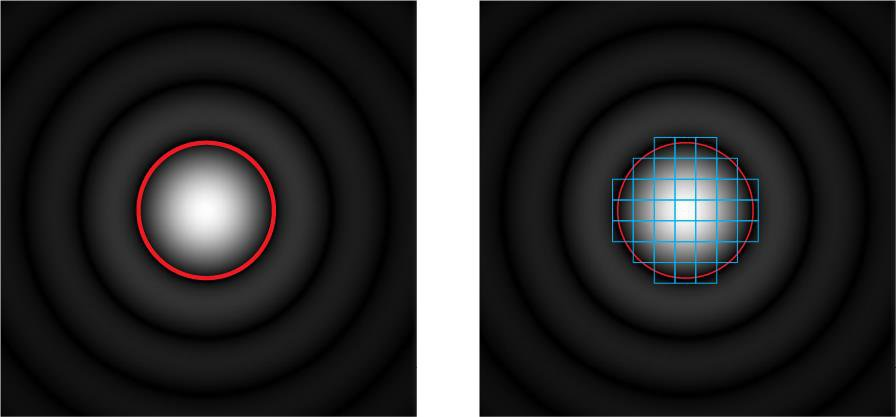
\includegraphics[width=\textwidth]{Fig/3.jpg}
        \caption{}
        \label{fig:pinhole_airy}
    \end{subfigure}

    \vspace{0.3cm}

    \begin{minipage}{0.7\textwidth}
        \centering
        \begin{subfigure}[b]{0.4\textwidth}
            \centering
            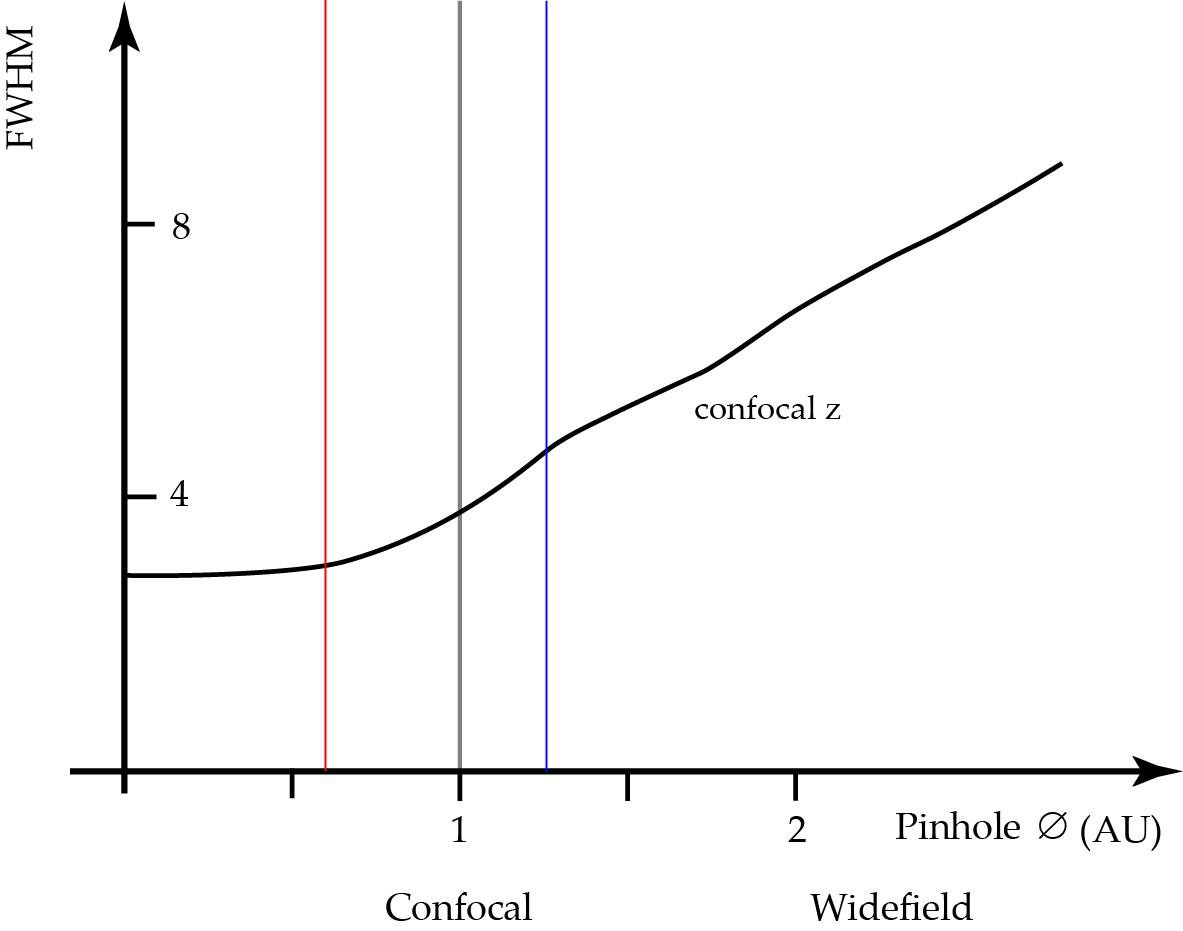
\includegraphics[width=\textwidth]{Fig/4.jpg}
            \caption{}
            \label{fig:pinhole_z}
        \end{subfigure}
        \hfil
        \begin{subfigure}[b]{0.4\textwidth}
            \centering
            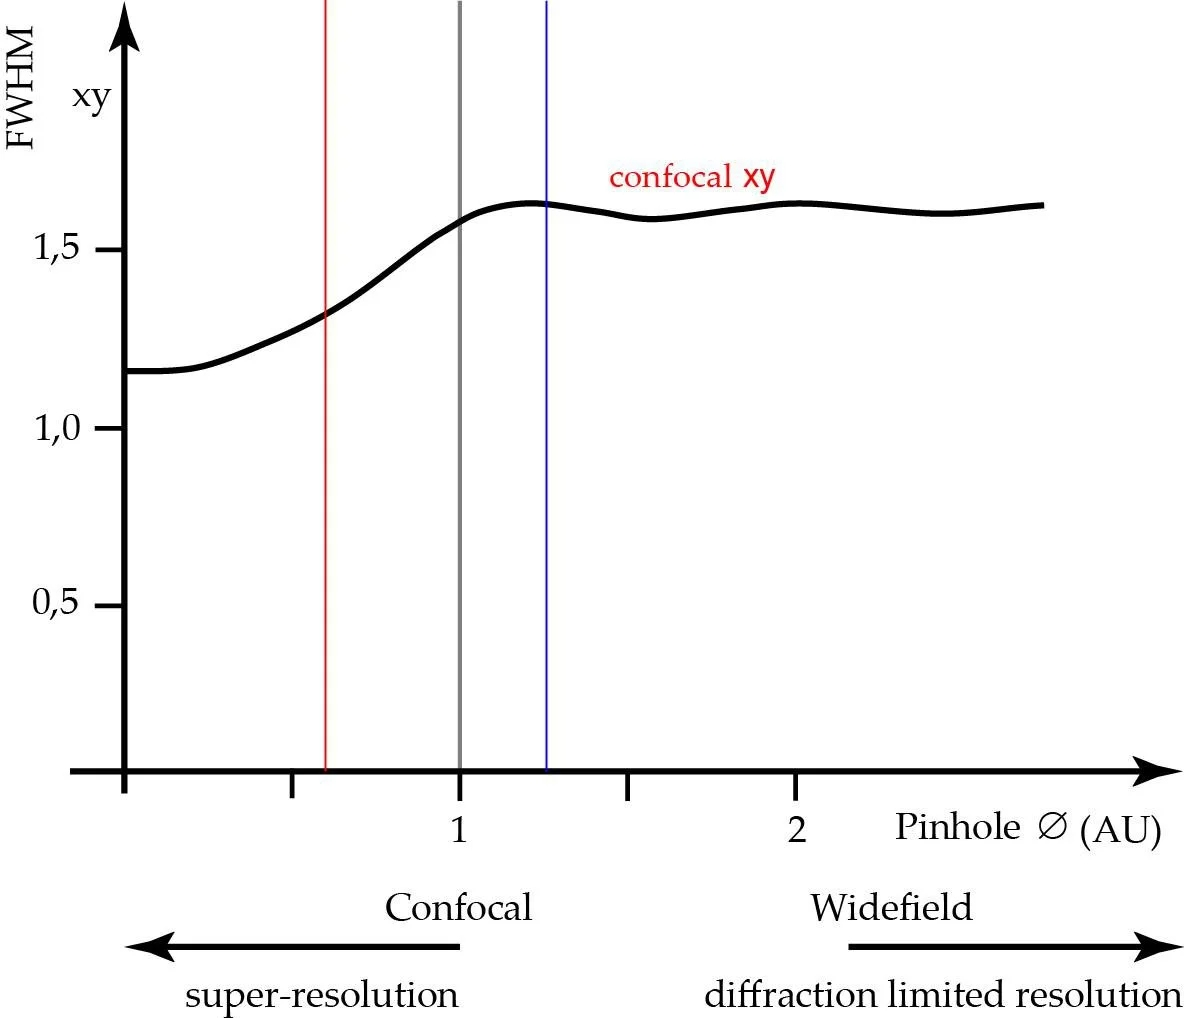
\includegraphics[width=\textwidth]{Fig/5.jpg}
            \caption{}
            \label{fig:pinhole_xy}
        \end{subfigure}
    \end{minipage}

    \bicaption{共焦小孔尺寸对共聚焦显微镜成像性能的影响。(a) 共焦小孔与艾里斑(Airy disk)的相对大小示意；(b) 轴向分辨率(FWHM$_z$)随小孔直径的变化；(c) 横向分辨率(FWHM$_{xy}$)随小孔直径的变化\cite{Leica}}{Influence of confocal pinhole size on confocal imaging performance. (a) Relative size of the confocal pinhole and the Airy disk; (b) axial resolution (FWHM$_z$) as a function of pinhole diameter; (c) lateral resolution (FWHM$_{xy}$) as a function of pinhole diameter\cite{Leica}}
    \label{fig:Leica}
\end{figure}

在前述激光扫描共聚焦显微镜中，系统能够区别于宽场成像的关键，不仅在于点扫描激发方式本身，更在于探测路径中引入了共焦小孔(pinhole)这一空间滤波元件。前文已经指出，共聚焦显微镜之所以能够获得优于宽场成像的对比度和轴向分辨率，本质上是由于其有效点扩散函数同时受到激发与探测过程的空间约束；而这种探测约束正是通过共焦小孔实现的。

对于位于焦平面附近的信号，其在探测共轭像面上能够形成较为集中的光斑，因此较容易通过小孔进入探测器；而来自离焦位置的荧光在该平面上的能量分布更为弥散，因而会被小孔部分或大部分阻挡。正是由于这种空间选择性，共聚焦显微镜能够显著抑制离焦背景，提高图像对比度，并增强系统的光学切片能力。

在工程上，共焦小孔的大小通常采用艾里单位(Airy unit, AU)表征。1 AU 通常对应于与理想艾里斑尺寸相当的小孔直径，因此常被作为共聚焦系统调节小孔大小时的重要参考尺度。图~\ref{fig:Leica}为共聚焦小孔对显微镜成像性能的影响，其中子图a为小孔和艾里斑相对尺寸示意图，子图b和c分别给出了轴向与横向分辨率随小孔直径变化的趋势。图~\ref{fig:Leica} 表明，小孔尺寸会同时影响系统的离焦抑制能力、空间分辨率和探测信号通量。

当小孔直径逐渐减小时，离焦信号受到更强抑制，系统的光学切片能力增强，轴向分辨率改善尤为明显；横向分辨率也会在一定范围内得到提升。这一趋势与前文关于共聚焦系统有效点扩散函数变窄的分析是一致的，即小孔越小，探测过程对焦点附近信号的选择性越强，从而使系统整体 PSF 进一步收缩。

然而，小孔并非越小越好。随着孔径继续减小，能够通过小孔的总荧光通量会迅速下降，导致探测信号减弱、信噪比降低，并可能迫使系统采用更高激发功率或更长积分时间来维持图像质量。对于生物荧光样品而言，这又会进一步增加光漂白和光毒性的风险。


\begin{figure}[htbp]
    \centering
    \begin{subfigure}[b]{0.75\textwidth}
        \centering
        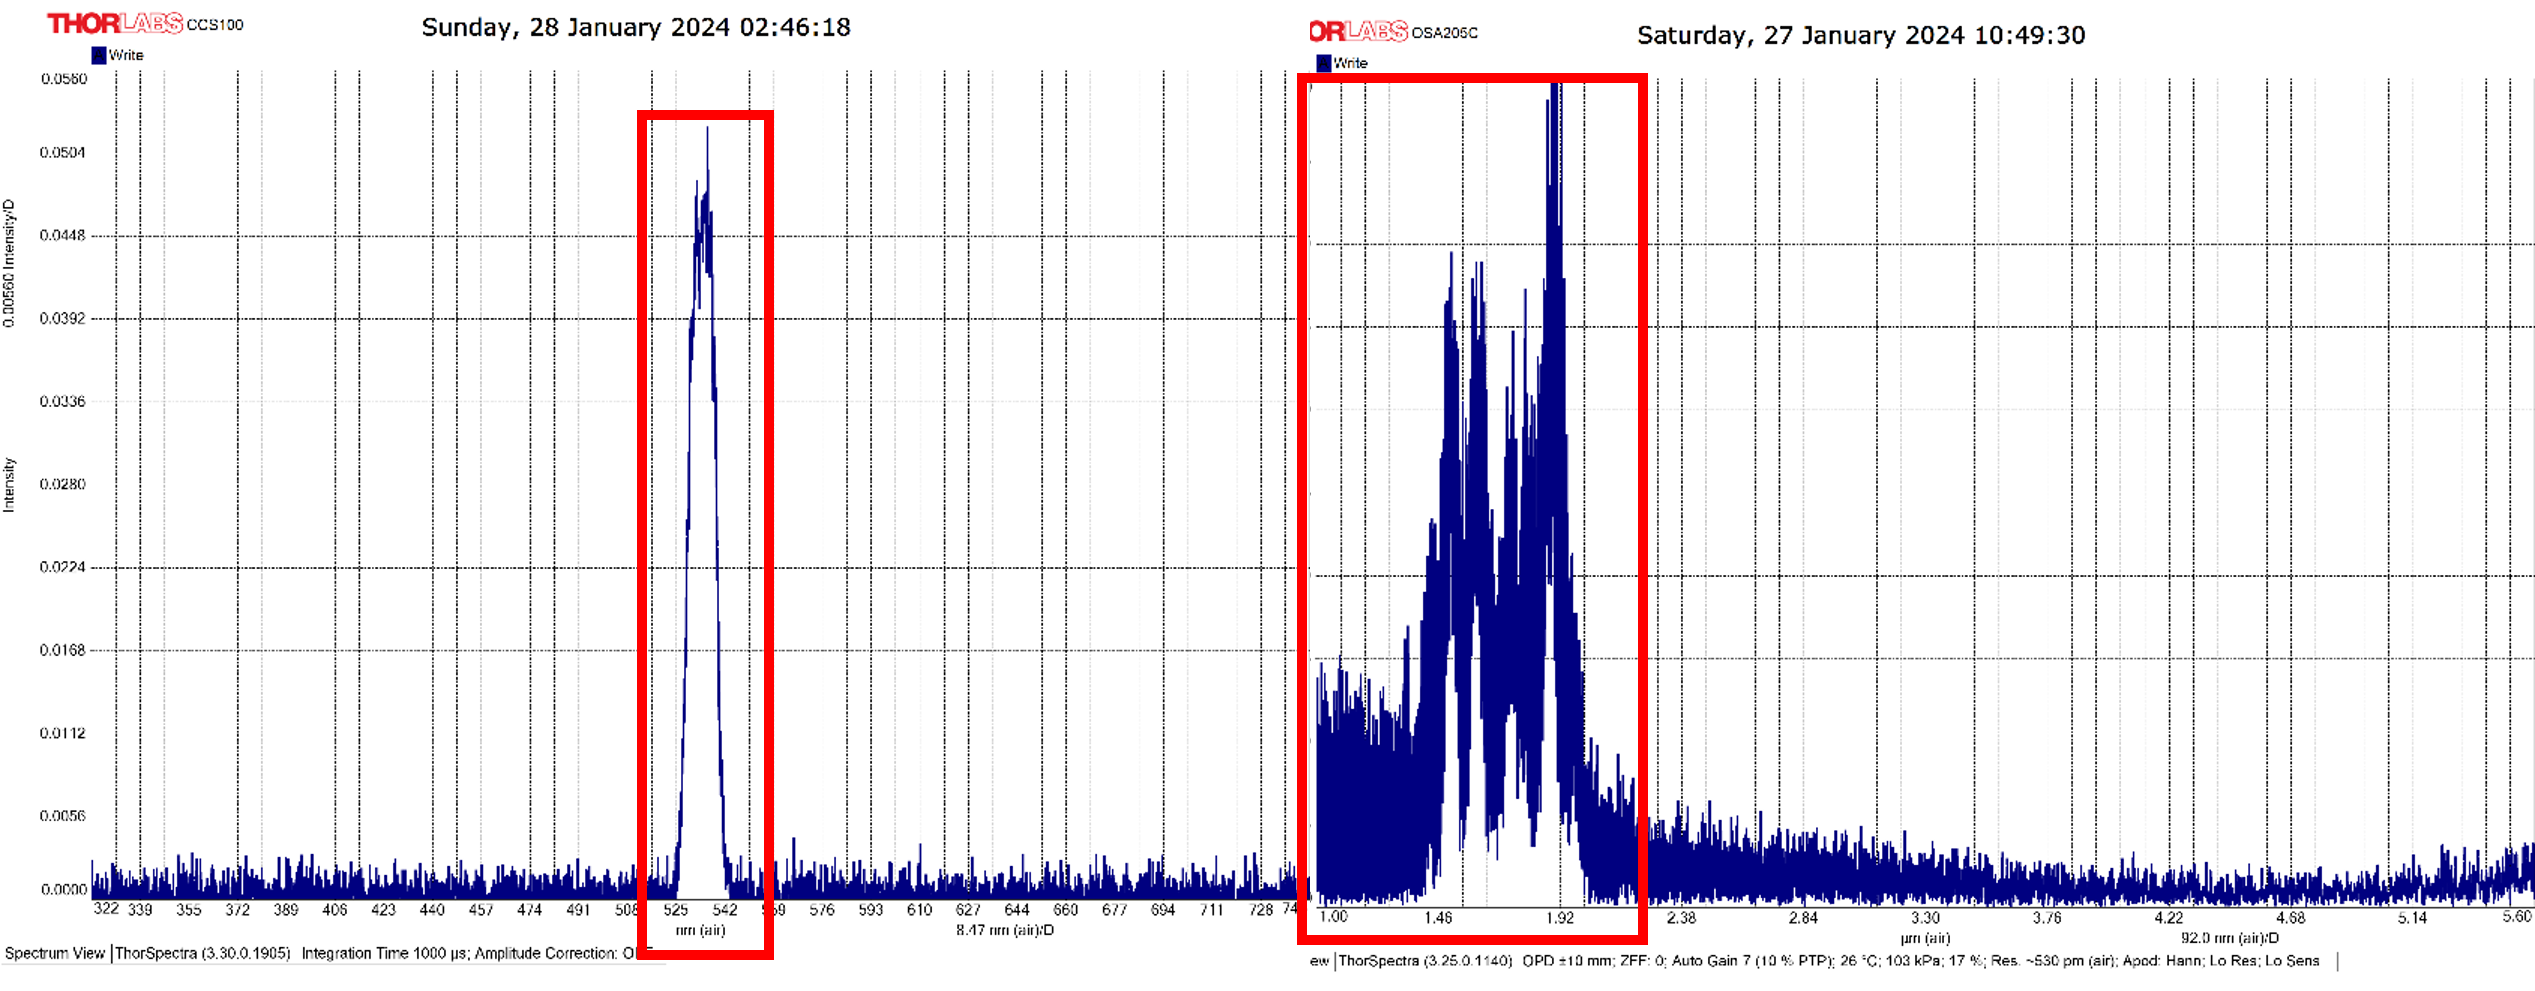
\includegraphics[width=\textwidth]{Fig/Fig34.png}
        \caption{}
        \label{fig34}
    \end{subfigure}

    \vspace{0.2cm}

    \begin{minipage}{0.8\textwidth}
        \centering
        \begin{subfigure}[b]{0.45\linewidth}
            \centering
            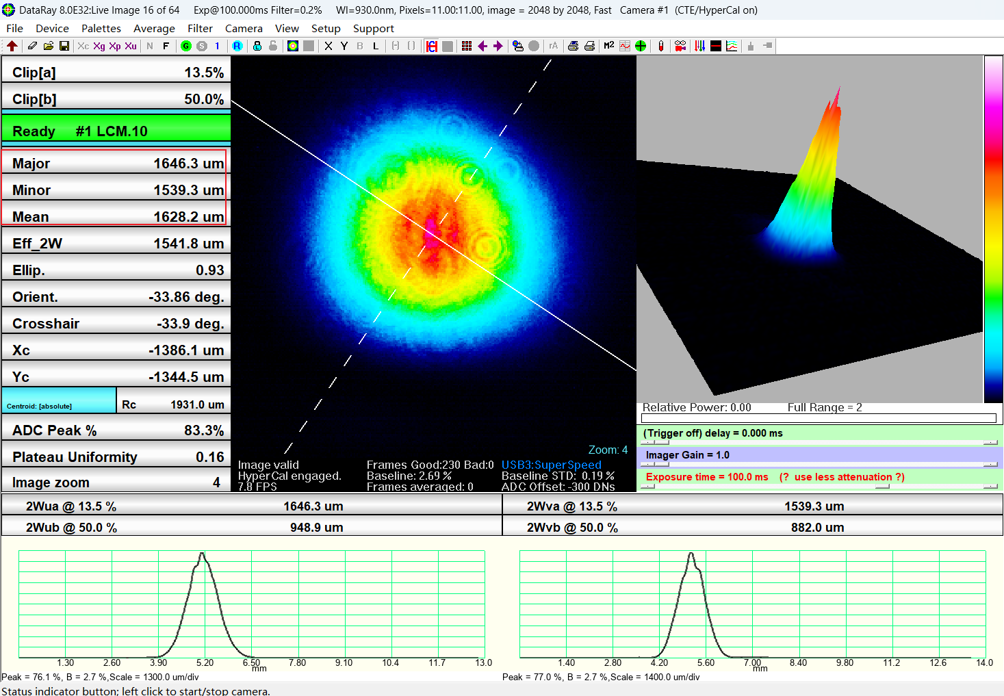
\includegraphics[width=\linewidth]{Fig/Fig36.png}
            \caption{}
            \label{fig36}
        \end{subfigure}
        \begin{subfigure}[b]{0.45\linewidth}
            \centering
            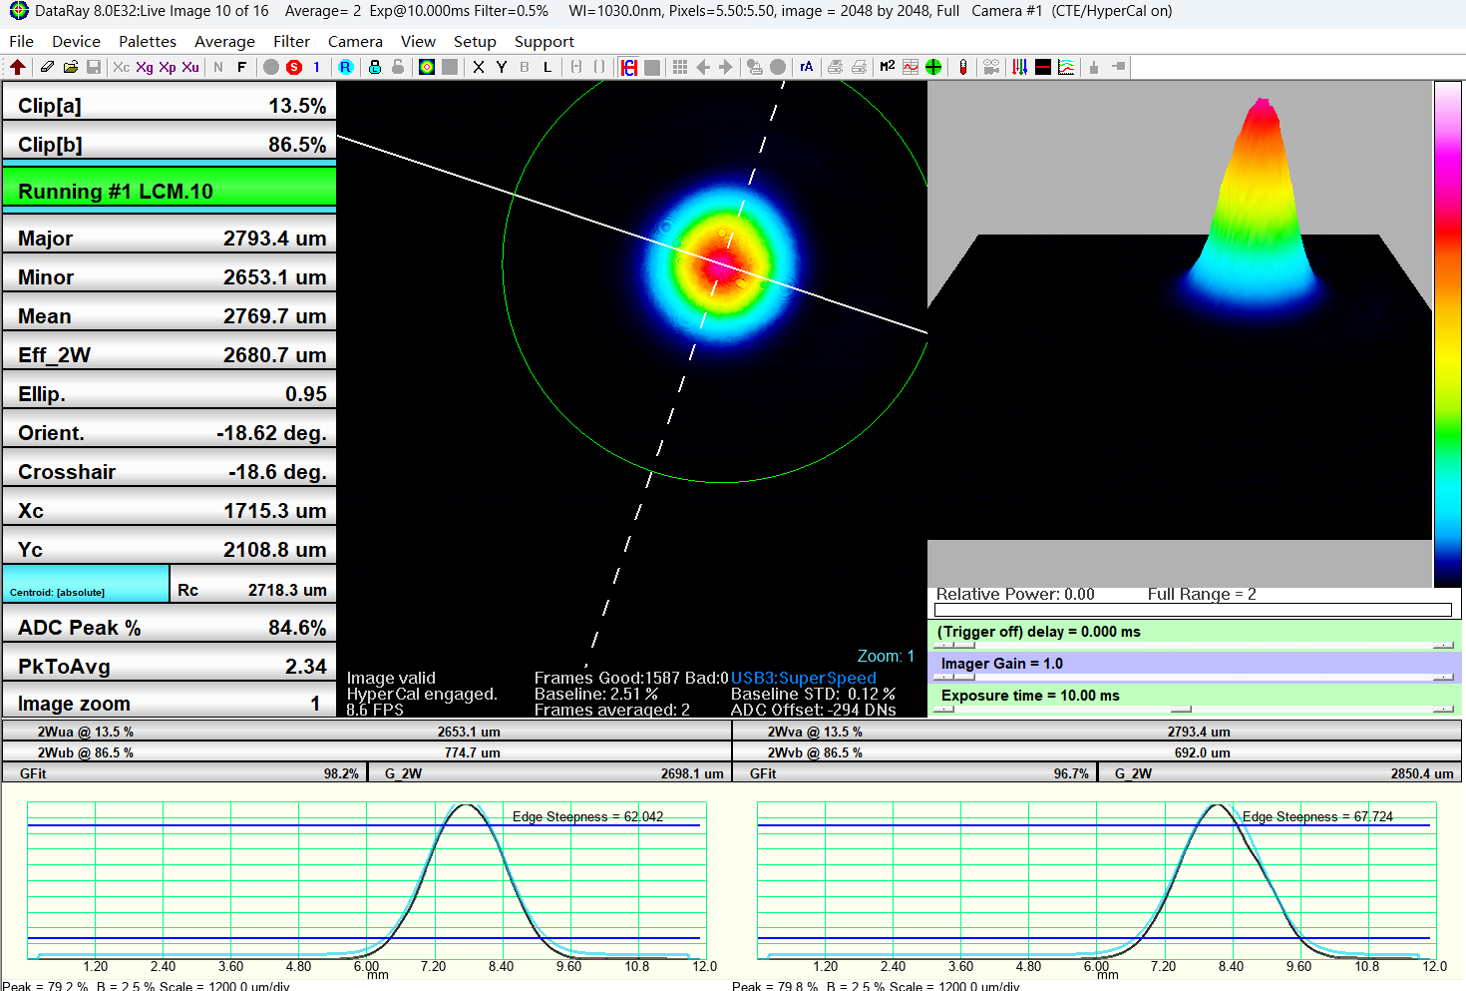
\includegraphics[width=\linewidth]{Fig/Fig35.png}
            \caption{}
            \label{fig35}
        \end{subfigure}
    \end{minipage}

    \bicaption{超连续谱激发光源的光谱整形与光束扩束结果。(a) 输出光谱；(b) 扩束前的光斑大小与形状；(c) 扩束后的光斑大小与形状}{Spectral shaping and beam-expansion results of the supercontinuum excitation source. (a) Output spectrum; (b) beam spot size and shape before expansion; (c) beam spot size and shape after expansion}
    \label{fig34-36}
\end{figure}

因此，在实际应用中，共焦小孔的设定通常需要在分辨率、光学切片能力与信号强度之间进行折中。对于大多数常规成像任务，将小孔设置在约 1 AU 附近通常能够在图像亮度与共聚焦效果之间取得较好的平衡；若进一步减小到 1 AU 以下，系统分辨率仍可能继续改善，但其代价往往是显著的信号损失，因此通常只在对空间分辨率要求较高且样品信号较强的条件下采用。

在散射较强的厚样品中，这一矛盾会更加突出。焦点处产生的有效荧光在传播过程中可能因散射而偏离原有传播方向，从而无法高效通过共焦小孔，导致有效信号进一步损失。尤其在紫外和可见光波段，生物组织对光的散射和吸收更为明显，因此共聚焦显微镜虽然在薄样品和透明样品成像中表现优异，但在厚组织深层成像时通常会受到穿透深度不足和信号迅速衰减的限制。这也是其在深层组织成像能力上通常不及双光子显微镜的重要原因之一。




\section{激发光源的光谱选择与光束整形}\label{3.2}

为满足多色共聚焦荧光寿命成像系统对不同激发波长和不同样品类型的需求，本文系统中配置了两类主要激发光源：一类为白光超连续谱激光器，用于提供可调谐的多波段激发；另一类为 532\,nm 皮秒激光光源，用于窄带单波长激发及荧光寿命测量相关实验。

\subsection{超连续谱激发光源的光谱选择与扩束}\label{3.2.1}

白光超连续谱激光器具有覆盖范围宽、波长选择灵活等优势，适合用于多色激发和不同荧光探针的适配实验。然而，由于其输出光谱较宽，直接用于显微激发时往往会引入不需要的波段成分，甚至造成额外背景和系统串扰，因此需要通过滤光片组合对目标波段进行选取和整形。


图~\ref{fig34-36}(\subref{fig34}) 给出了超连续谱激光器经过 488/10 带通滤光片与热反射镜(Hot Mirror)滤波后的输出光谱。可以看出，经过初步滤波后，目标激发波段得到了有效保留，但在 1100\,nm 以上仍存在残余干扰成分。为进一步抑制该部分长波背景，系统中加入了 1035\,nm 短通滤光片(麓邦光学)进行进一步滤除，从而提高了目标波段的纯净度，降低了非目标波长进入显微系统后可能造成的背景干扰。

除光谱选择外，激发光束的空间形态也直接影响后续扫描系统中的束径填充和聚焦质量。图~\ref{fig34-36}(\subref{fig36}) 和图~\ref{fig34-36}(\subref{fig35}) 分别给出了超连续谱光源在扩束前后的光斑大小与形状对比。扩束前，光束直径较小，不利于后续在物镜后孔径处实现充分填充；扩束后，激发光束尺寸得到放大，更有利于与前文所述的物镜后孔径尺寸匹配，从而提高有效激发数值孔径并改善聚焦效果，扩束设计请参考第\ref{2.4.2}小节。


% 因此，对于超连续谱激发光源而言，其在显微系统中的关键并不仅仅是``能否出光''，而在于能否通过合适的滤波与扩束方案，获得满足目标波段、功率密度和空间束形要求的稳定激发光。这对于后续多色共聚焦成像和寿命测量具有基础性作用。


\subsection{532nm 皮秒激光光源及其系统适配}\label{3.2.2}

除超连续谱光源外，本文系统还采用了 532\,nm 皮秒激光器(朗研光学)作为另一类重要激发光源。与宽谱超连续谱光源相比，532\,nm 皮秒光源具有波长单一、输出稳定、脉冲参数明确等特点，尤其适用于需要固定激发波长和时间分辨探测的实验场景，例如特定荧光染料的激发和荧光寿命成像中的同步测量。特别是其单脉冲能量非常高，适合低重频下同时激发染料的多个光子，对于光子计数的lifetime研究非常合适。

在系统实现中，532\,nm 光源同样需要经过功率调节、准直与扩束后进入扫描显微镜光路。其功率大小直接影响样品处的激发效率和最终荧光信号强度；若功率过低，则难以获得足够信噪比，若功率过高，则可能导致荧光样品发生光漂白甚至光损伤。因此，在实验中通常需要结合样品荧光强度、探测器灵敏度以及扫描速度对 532\,nm 激发功率进行合理设定。

此外，由于 532\,nm 光源同时具备较好的单色性和较稳定的脉冲输出，因此在系统调试过程中还可作为重要的基准激发源，用于验证激发光路耦合状态、扫描对准情况以及探测链路响应。与超连续谱光源相比，532\,nm 皮秒激光器更适合用于稳定性要求较高的定点实验和寿命测量实验，而超连续谱光源则在多波段灵活激发方面更具优势。二者在本文构建的共聚焦荧光寿命成像系统中形成了互补关系。



\section{系统设计}\label{3.3}

在前文对共聚焦显微技术基本原理、共焦小孔作用以及激发光源配置进行分析的基础上，本节进一步介绍自主搭建的共聚焦显微成像系统的具体设计方案与演进过程。为了满足后续多通道荧光成像与荧光寿命探测的实验需求，系统总体设计遵循``由简到繁、由单一功能到模块化扩展''的迭代思路：首先完成基础共聚焦光路的搭建与验证，在此基础上逐步加入多色激发、分路探测和可更换滤波模块，最终形成一套兼顾稳定性、扩展性与可维护性的多通道共聚焦显微成像平台。



\subsection{共聚焦系统原型的迭代演进}

系统的光路设计经历了四个主要阶段的演进，如图~\ref{fig:fig30_32} 所示。最初版本采用白光超连续谱激光器配合带通滤波片作为激发源，以验证共聚焦激发、扫描和信号收集链路的基本可行性。

\begin{figure}[htbp]
    \centering

    \begin{subfigure}[b]{0.48\textwidth}
        \centering
        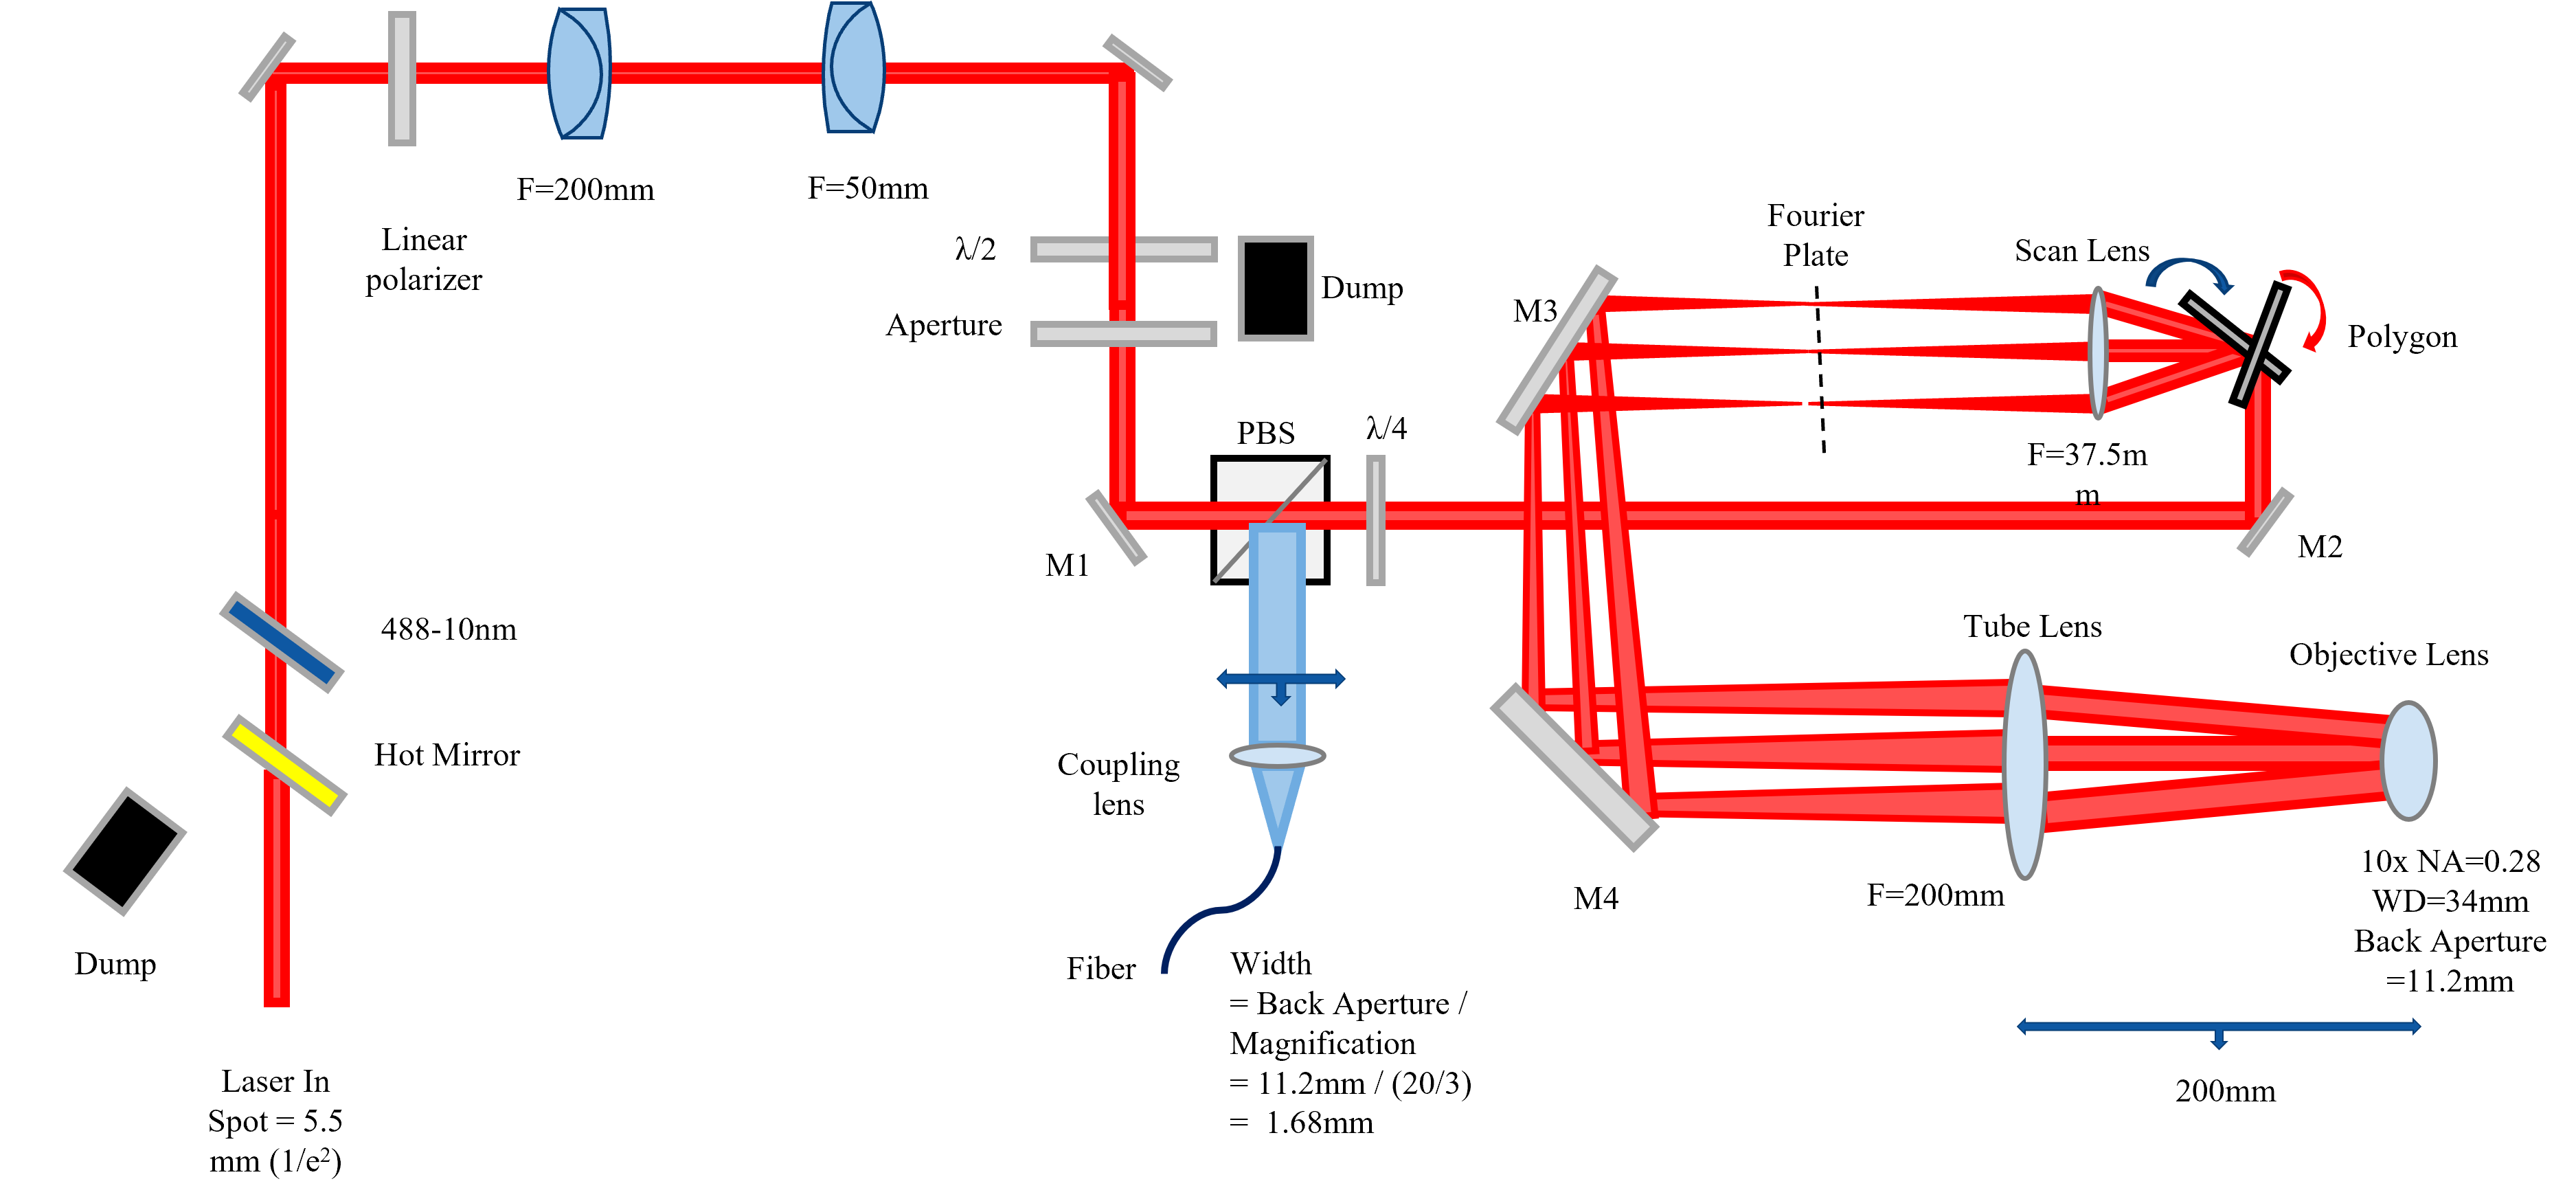
\includegraphics[width=\textwidth]{Fig/Fig30.png}
        \caption{}
        \label{fig:fig30}
    \end{subfigure}
    \hfill
    \begin{subfigure}[b]{0.48\textwidth}
        \centering
        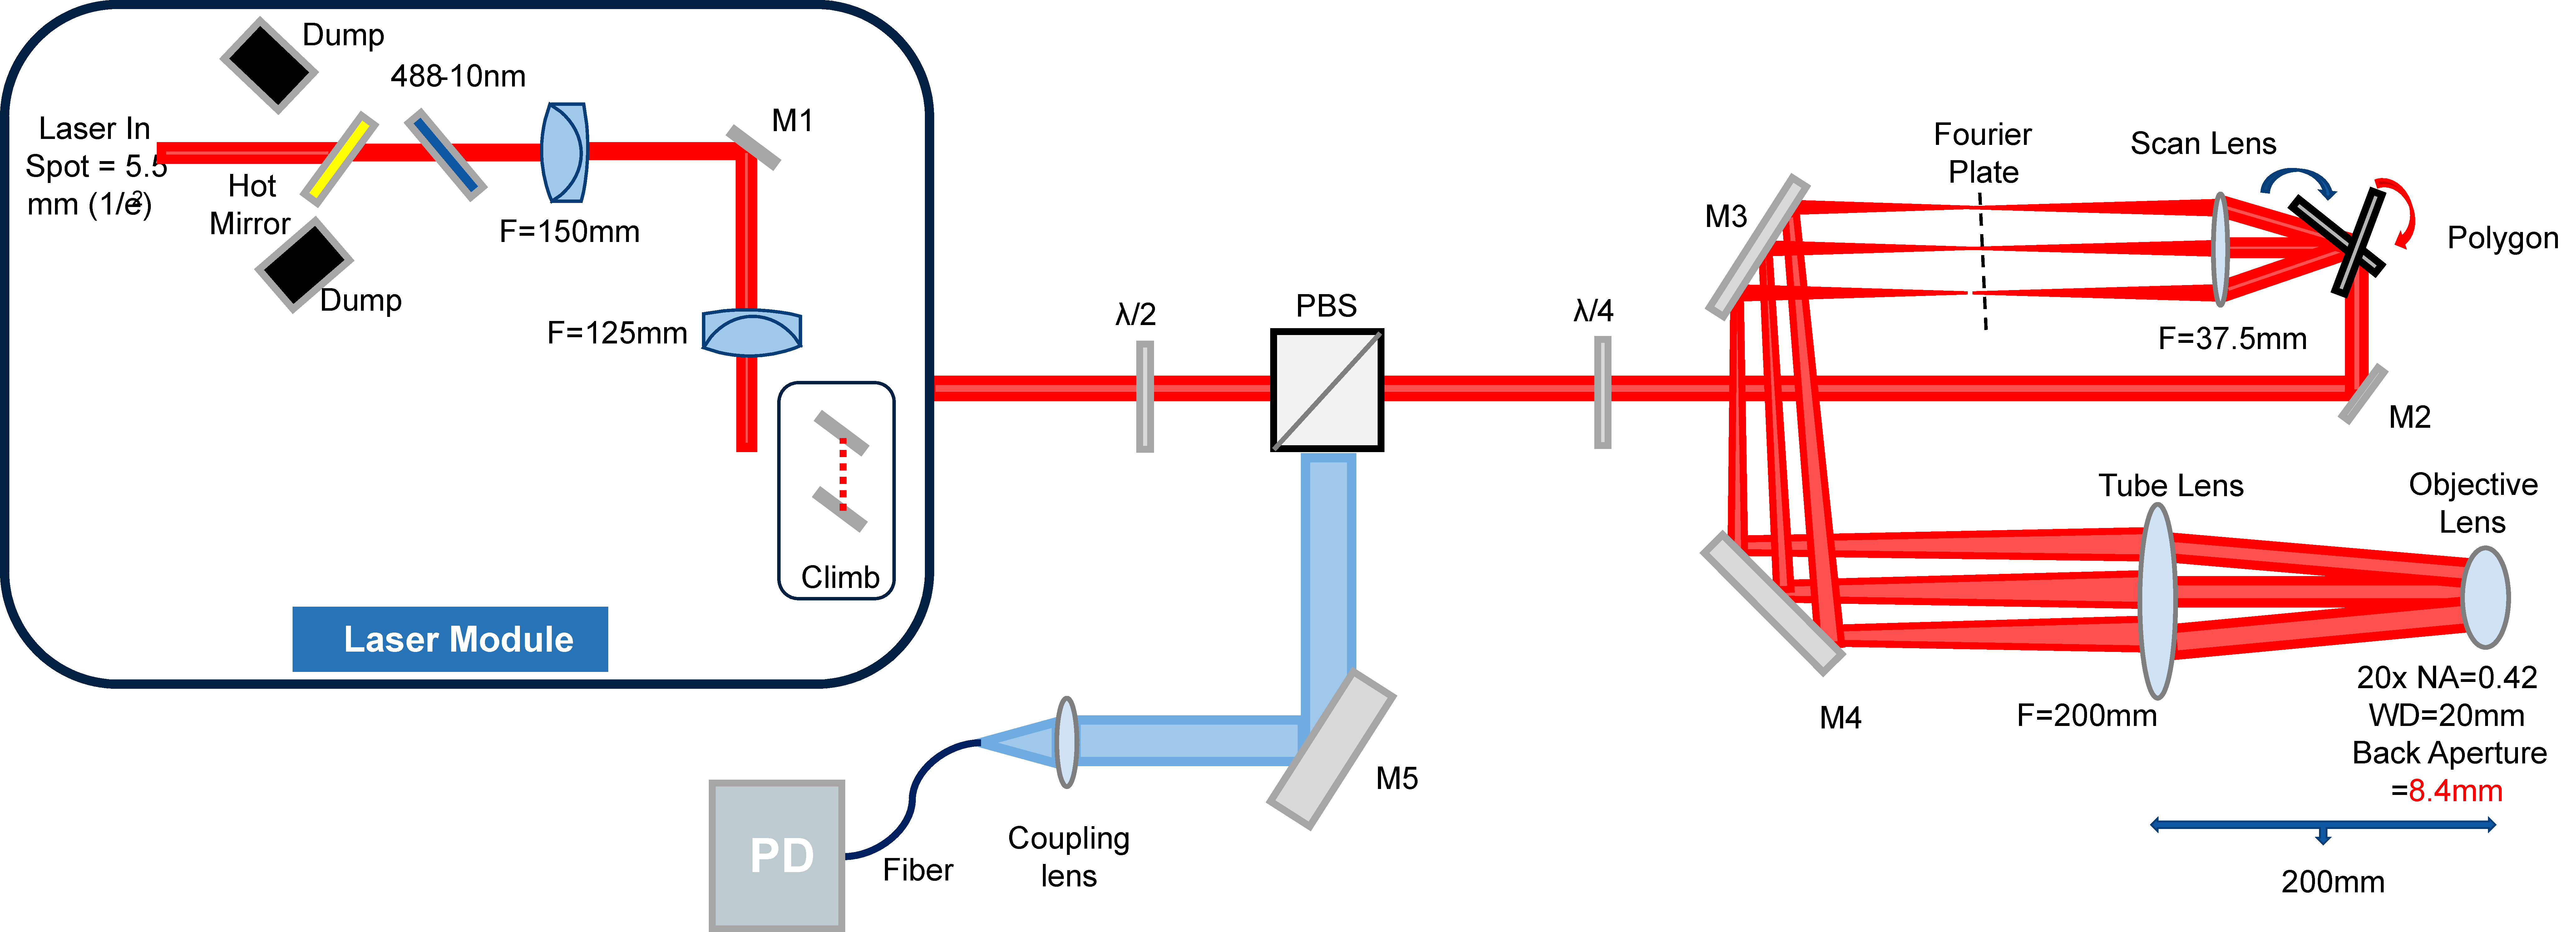
\includegraphics[width=\textwidth]{Fig/Fig31.pdf}
        \caption{}
        \label{fig:fig31}
    \end{subfigure}

    \vspace{0.5cm}

    \begin{subfigure}[b]{0.48\textwidth}
        \centering
        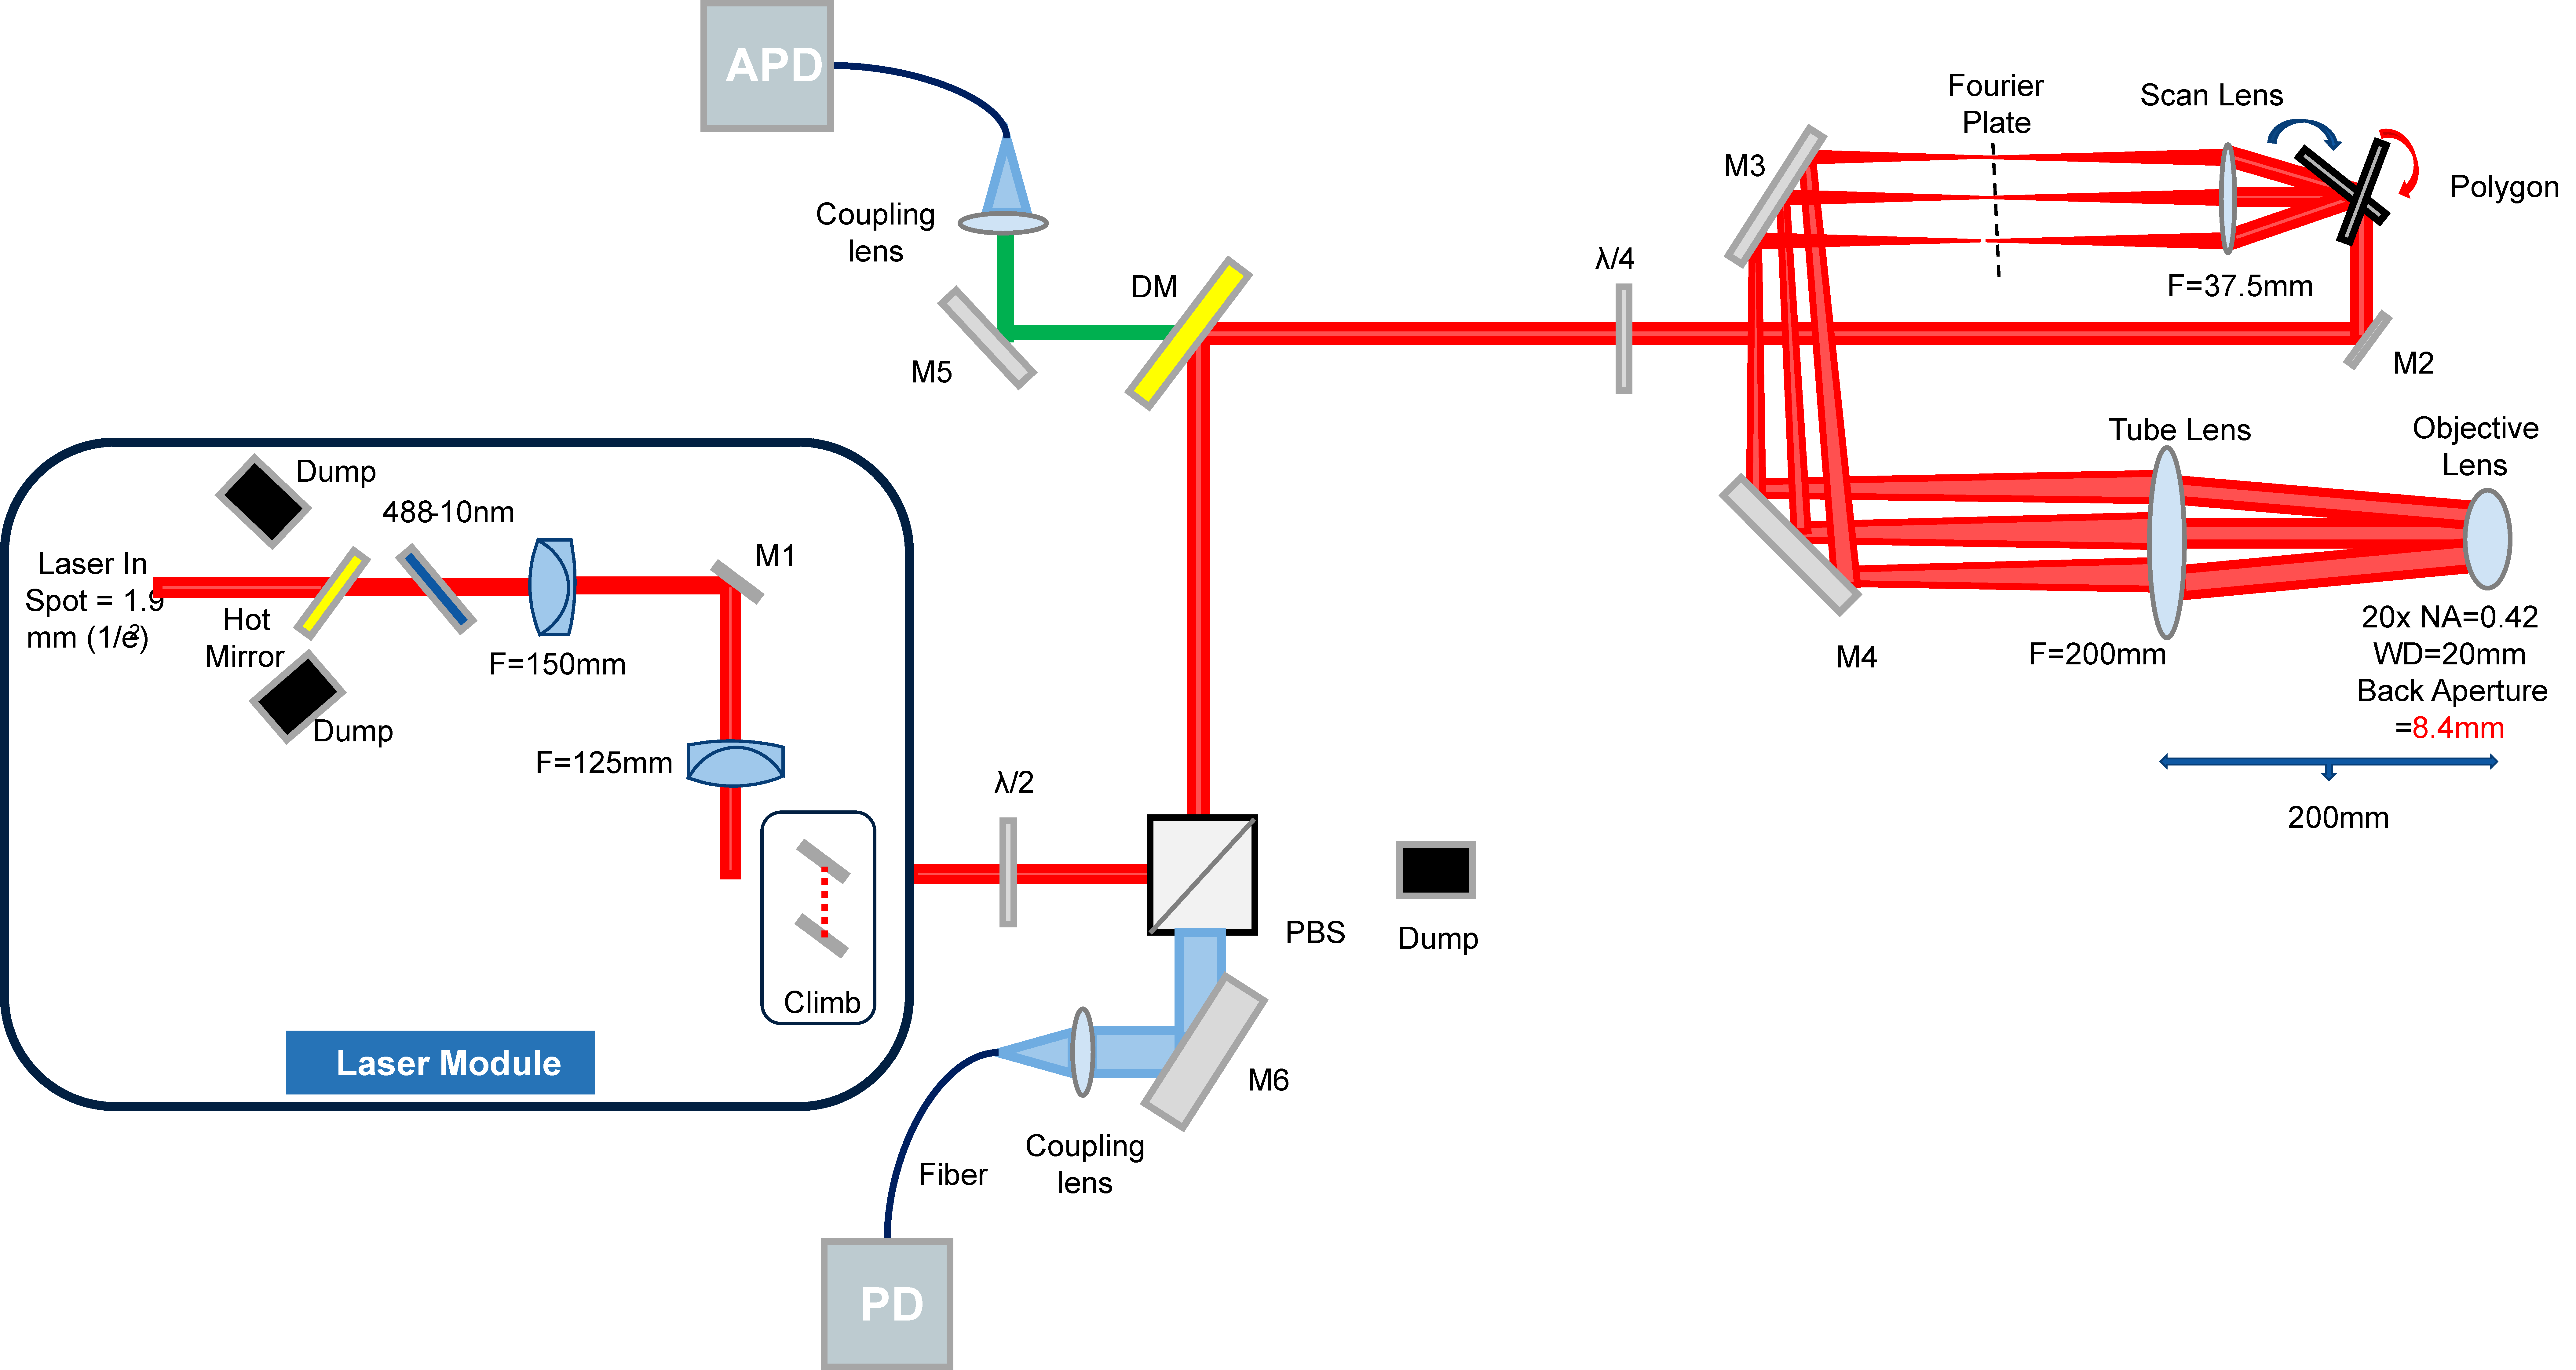
\includegraphics[width=\textwidth]{Fig/Fig31.5.pdf}
        \caption{}
        \label{fig:fig31_5}
    \end{subfigure}
    \hfill
    \begin{subfigure}[b]{0.48\textwidth}
        \centering
        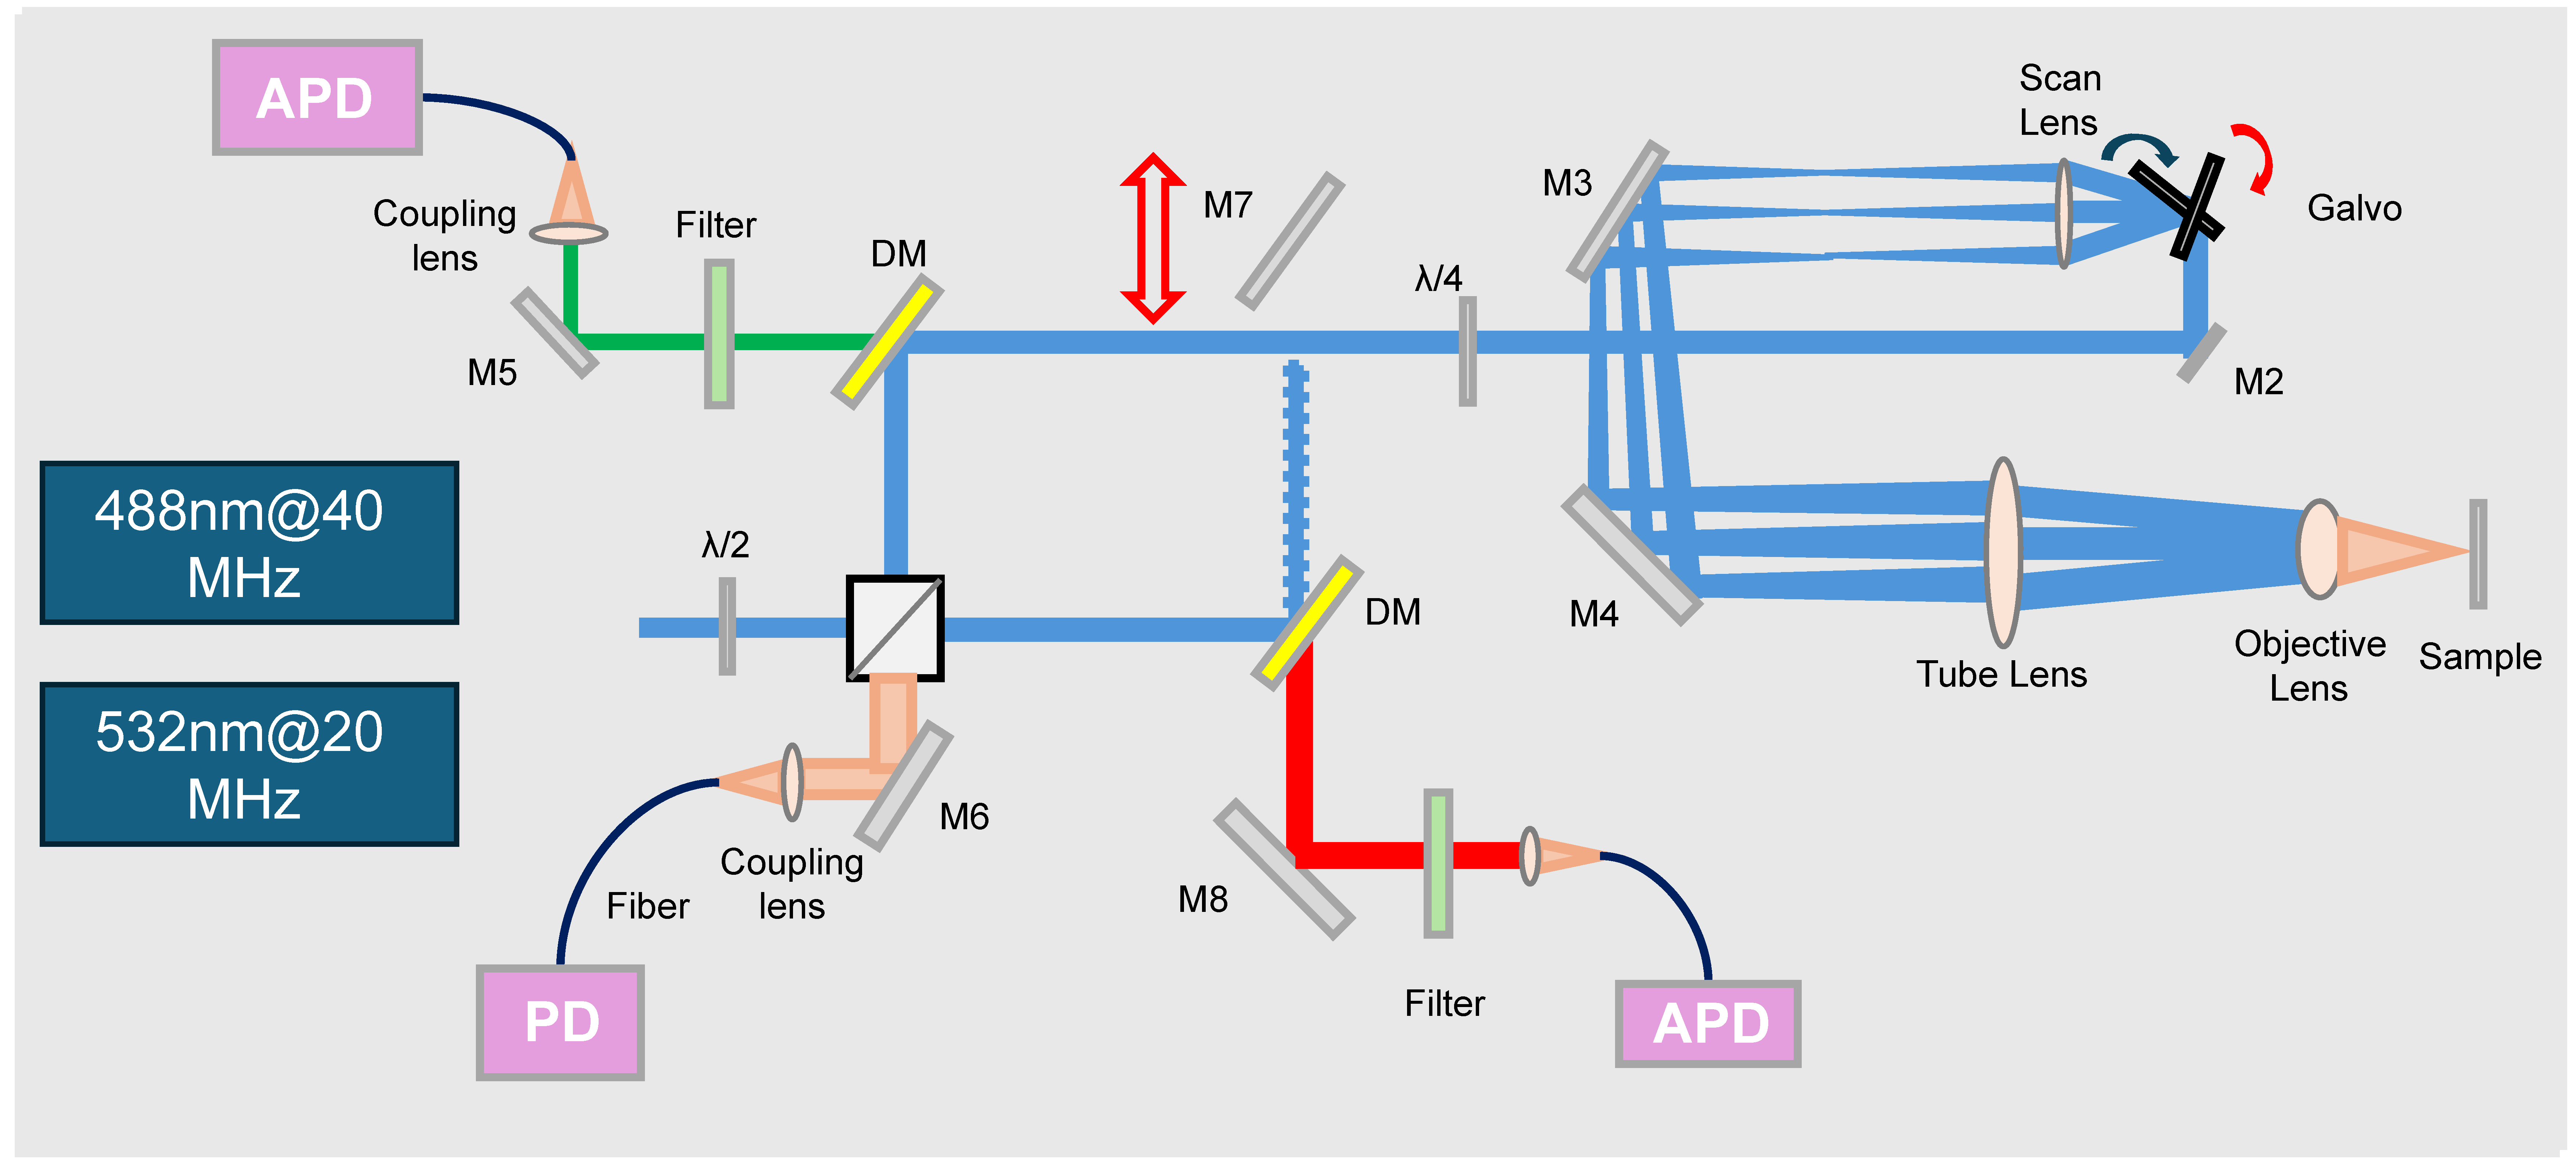
\includegraphics[width=\textwidth]{Fig/Fig32.pdf}
        \caption{}
        \label{fig:fig32}
    \end{subfigure}

    \bicaption{共聚焦系统演进过程。(a) 白光超连续共聚焦系统第一版；(b) 白光超连续共聚焦系统第二版；(c) 白光超连续共聚焦系统第三版；(d) 白光超连续共聚焦系统第四版}{Evolution of the confocal system. (a) First-generation white-light supercontinuum confocal system; (b) second-generation system; (c) third-generation system; (d) fourth-generation system}
    \label{fig:fig30_32}
\end{figure}

第一版系统(图~\ref{fig:fig30_32}(\subref{fig:fig30}))采用一体化布局，构建了最基本的激发、扫描与反射式成像光路，用于验证系统准直、样品照明和信号回传链路是否可行。该版本实现了基础光路闭环，但在实际调试中暴露出明显不足：一旦需要切换光源或重新调整激发路径，往往会对后续显微镜主光路的准直状态造成影响，系统稳定性较差。

针对这一问题，第二版系统(图~\ref{fig:fig30_32}(\subref{fig:fig31}))在结构上采用分体式设计，将光源调制模块与显微镜主体光路在同一光学平台上相对独立布置，实现了激发模块与显微模块的空间解耦。该设计显著降低了更换光源和调节滤波模块时对主光路造成的扰动，提高了系统的调试效率与重复性。

在此基础上，第三版系统(图~\ref{fig:fig30_32}(\subref{fig:fig31_5}))进一步引入了 532\,nm 特定波长激发模块，使系统不仅能够使用超连续谱光源进行多波段激发，还具备了稳定的单色荧光激发能力，为后续荧光寿命成像和特定染料激发实验提供了更加明确的光源条件。

最终，经过前述多个阶段的迭代优化，第四版系统(图~\ref{fig:fig30_32}(\subref{fig:fig32}))实现了双路激发以及``双路荧光/单路反射''共三种探测通道的集成。通过合理配置二向色镜与发射滤光片，系统能够根据实验需求在不同激发与探测模式之间进行切换，从而满足多色共聚焦成像及后续荧光寿命探测的需求。相比初始版本，该阶段系统已经从单一验证型原型发展为具备较强扩展性的模块化共聚焦显微平台。



\subsection{最终系统光路设计与实现}

在完成原型迭代后，本文进一步搭建了最终版共聚焦显微成像系统，其光路原理如图~\ref{fig3P14} 所示。该系统在保留基础点扫描共聚焦结构的同时，将激发模块、扫描模块、显微物镜模块以及探测模块进行了统一整合，从而形成一套可用于多色荧光成像和寿命探测的完整实验平台。

\begin{figure}[htbp]
    \centering
    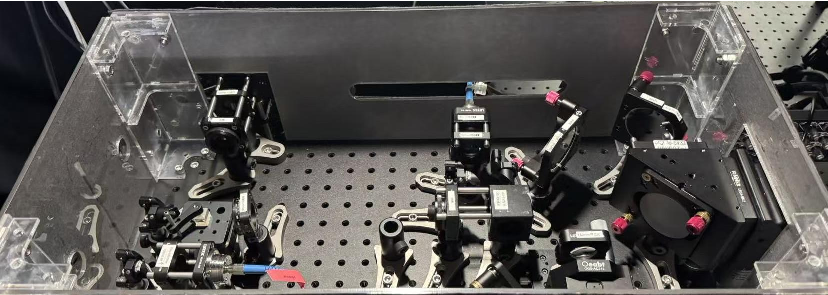
\includegraphics[width=\textwidth]{Fig/Fig3P14}
    \bicaption{实际搭建系统图}{Photograph of the assembled system}
    \label{fig3P14}
\end{figure}


在激发端，系统既可接入40MHz 的白光超连续谱激光器并通过带通滤波选择目标激发波段，也可接入单一波长的 20\,MHz、532\,nm 皮秒激光器作为稳定激发源。前者适用于多色激发与不同荧光探针的灵活适配，后者则适用于固定波长激发和后续时间分辨测量实验。无论采用哪种激发光源，激发光均经扩束、准直和扫描系统后进入显微镜主体，并最终由物镜聚焦到样品上。

在探测端，样品产生的反射光和荧光信号沿原光路返回，经分光元件分离后分别进入相应的探测通道。通过引入多路滤光片和二向色镜组合，系统能够根据激发波段和目标发射波段配置相应的荧光探测路径，并保留反射信号通道作为基准参考。该设计保证了系统在多色激发条件下仍具有良好的信号区分能力和较高的灵活性。

需要说明的是，本文利用 532\,nm 皮秒激光器对系统进行了初步成像验证，具体成像结果将在第\ref{5.5}节给出。该单色激发实验所采用的系统结构与图~\ref{fig:fig32} 和图~\ref{fig3P14} 所示原理一致，因此可视为最终系统设计在固定波长激发条件下的一种工作模式。



\subsection{磁吸式快拆多色共聚焦机械结构设计}

为将前述复杂的多通道多色荧光共聚焦系统转化为稳定可靠的实体装置，本文在光学设计之外，进一步采用 SolidWorks 完成了系统机械结构的精密建模与模块化设计，如图~\ref{fig37-46} 所示。相较于传统直接搭建在面包板上的开放式结构，该设计更加关注切换过程中的重复定位精度、机械稳定性以及维护便利性。

\begin{figure}[htbp]
    \centering
    \begin{subfigure}[b]{0.5\textwidth}
        \centering
        \includegraphics[width=\textwidth]{Fig/Fig37.png}
        \caption{}
        \label{fig37}
    \end{subfigure}
    \begin{subfigure}[b]{0.4\textwidth}
        \centering
        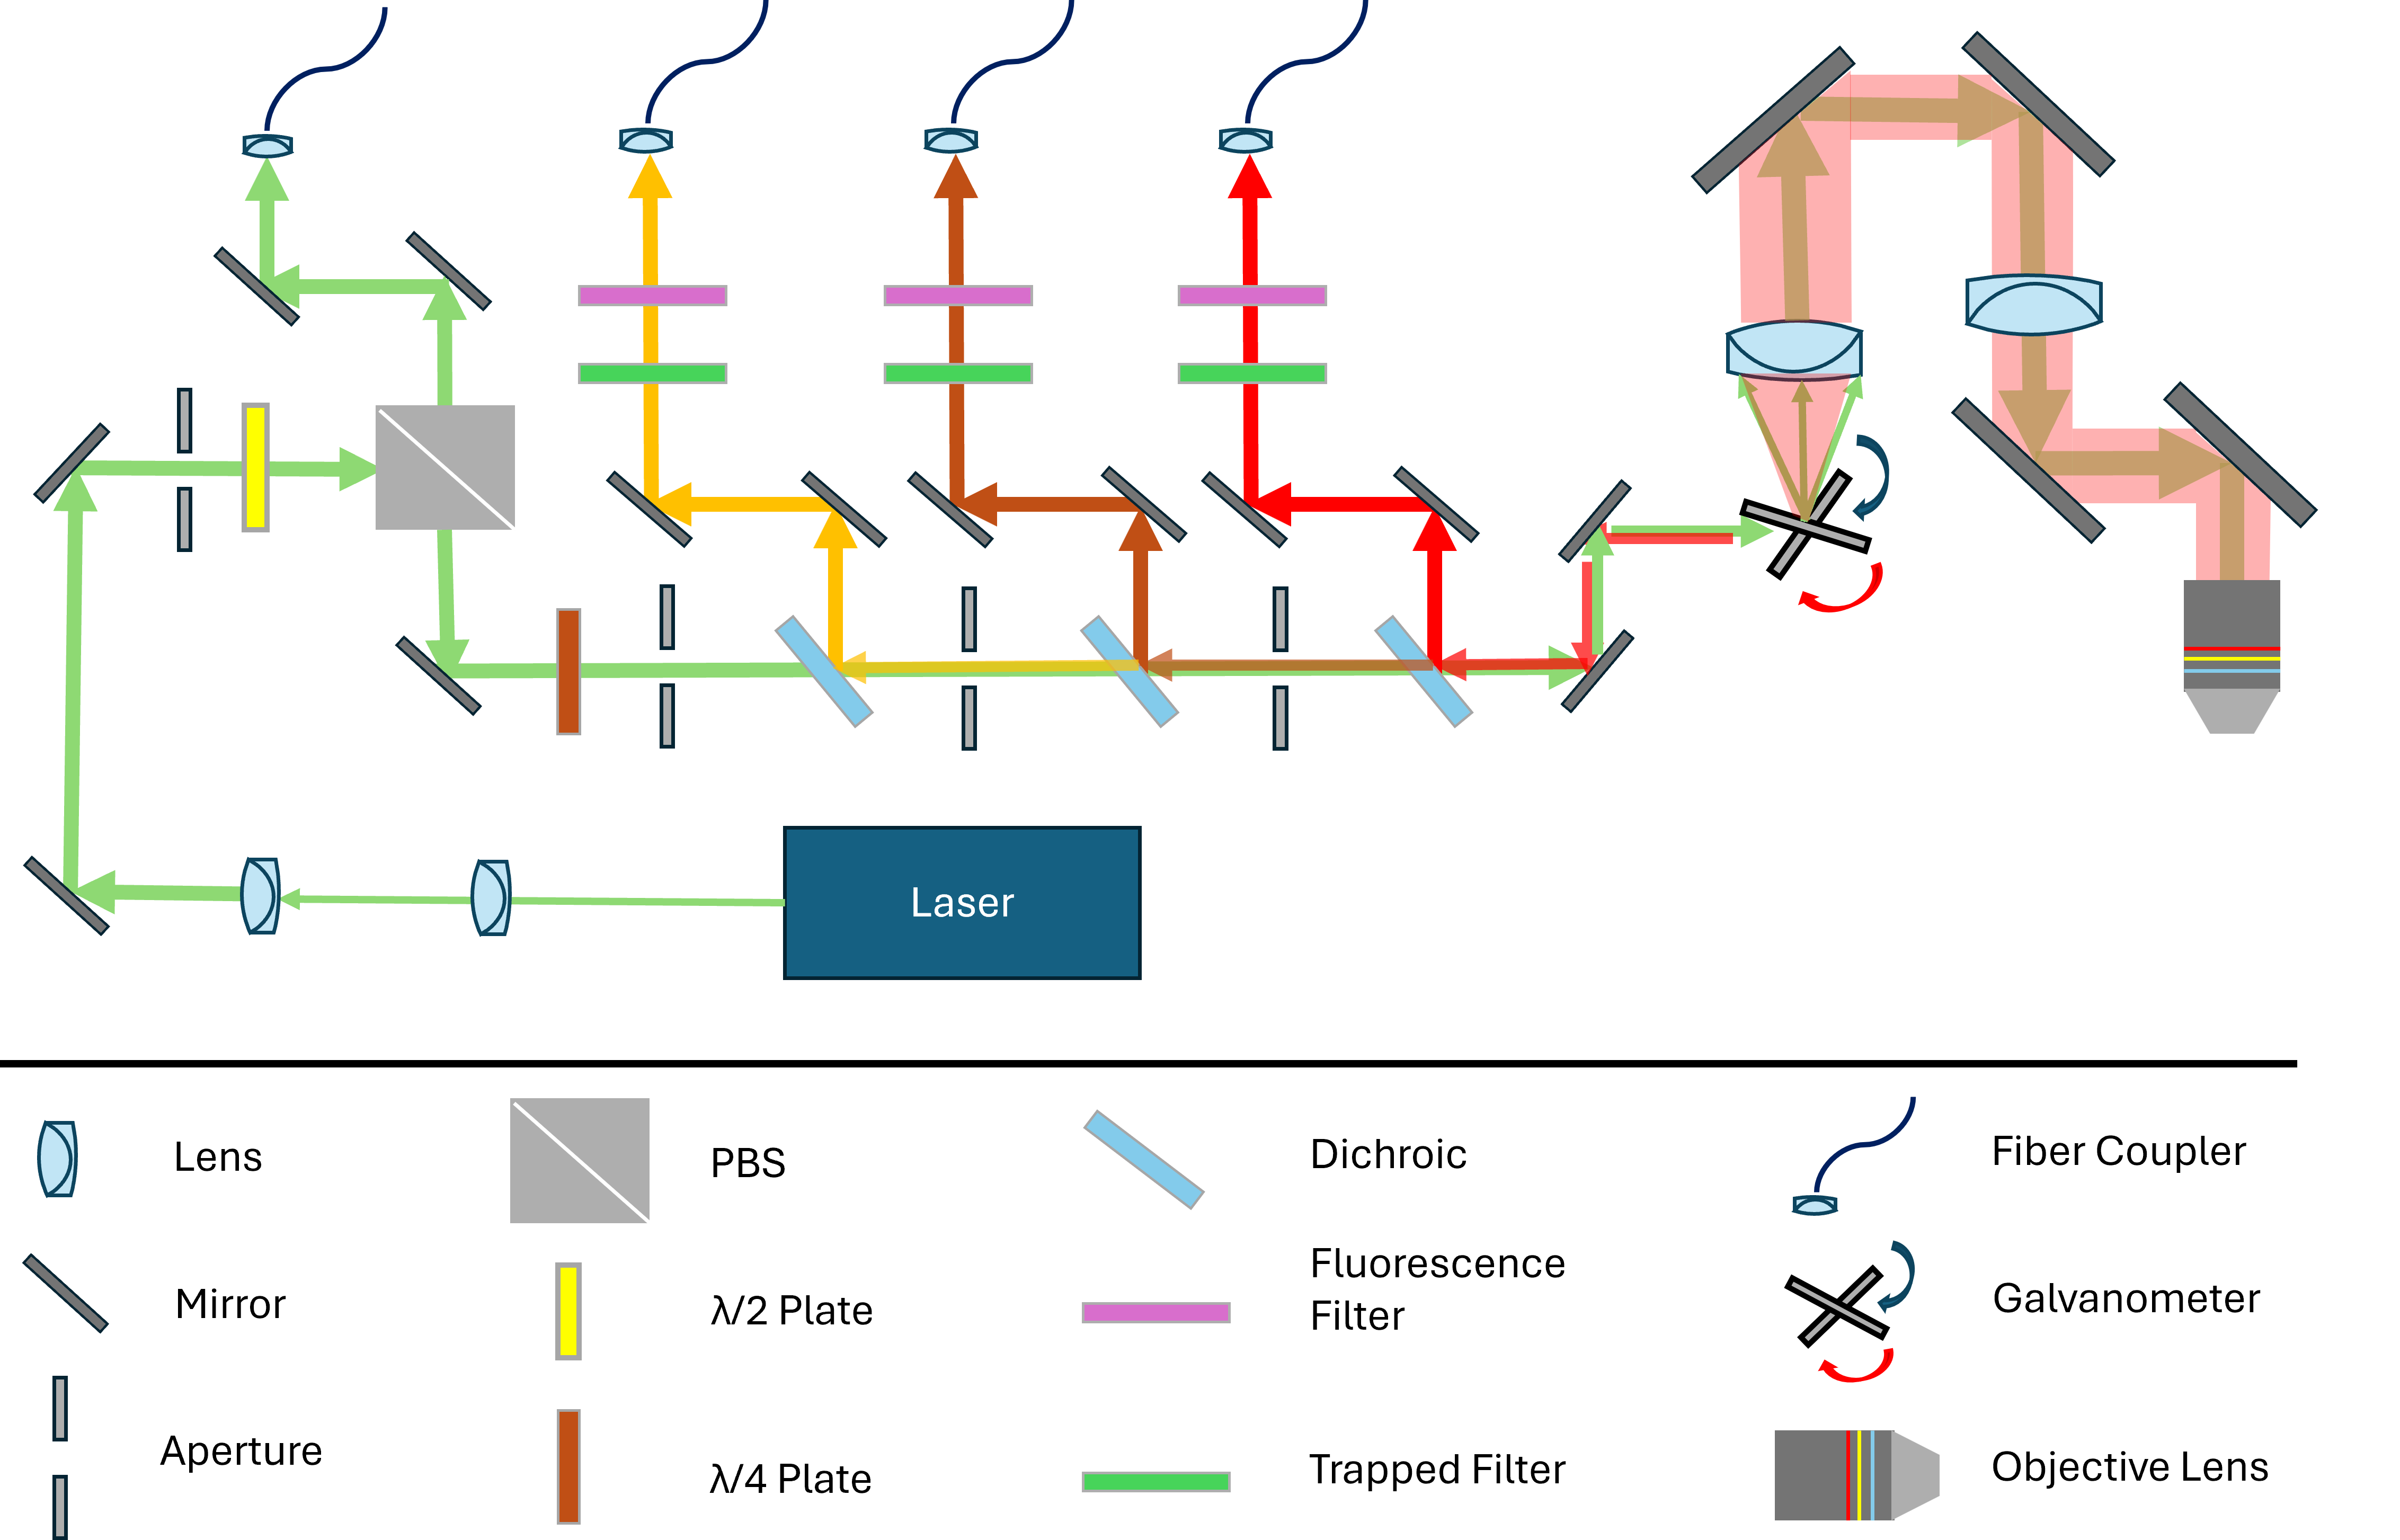
\includegraphics[width=\textwidth]{Fig/Fig46.png}
        \caption{}
        \label{fig46}
    \end{subfigure}
    \bicaption{可扩展的磁吸插入式多通道荧光共聚焦显微镜机械设计。(a) 基于 SolidWorks 的机械结构建模；(b) 系统模块化结构示意图}{Mechanical design of an extensible magnetic plug-in multichannel fluorescence confocal microscope. (a) Mechanical structural modeling based on SolidWorks; (b) schematic of the modular system architecture}
    \label{fig37-46}
\end{figure}

本设计于开发了一套``磁吸插入式''模块结构，用于实现激发滤光片、二向色镜和发射滤光片等关键光学元件的快速切换。相较于传统螺纹固定或滑轨式结构，磁吸式模块在频繁更换滤光片组件时具有更好的重复定位能力：模块在插入后可借助磁吸结构实现快速自定位，从而降低反复插拔过程带来的机械位移误差。更重要的是，该设计避免了每次更换滤波组件后都重新调整主光路，大幅提高了系统在多色实验中的切换效率。

此外，该结构基于定制化面包板与分层模块布局，可根据实验需求灵活增加或减少探测通道，具有较好的扩展性。对于需要同时兼顾多色激发、反射成像和荧光寿命探测的系统而言，这种兼顾稳定性与灵活性的机械设计具有明显优势。

同时，就磁吸式切换结构的重复使用及切换后的光路对准问题，我们分别在系统入光口设置一个3mm的固定光阑、在振镜入口处设置了一个可调光阑，以及在管透镜和扫描透镜中间焦距傅里叶面处放置一个大的孔径光阑，保证全部打开时不会影响信号采集。这三个光阑位置绝对固定不会影响磁吸模块切换或调整位置。

以及如图~\ref{fig37-46}(\subref{fig37}) 所示，所有光阑的前方均有一组(两个)反射镜，用于光路准直与调节(激光入光口处未画出)，以确保系统快速切换后可以保持良好的光路对准状态，避免每次更换滤波组件后都需要重新调整主光路，通过微调反射镜组件可以迅速找到准直状态，从而提高系统在多色实验中的切换效率和稳定性。


\begin{figure}[htbp]
    \centering

    \begin{subfigure}[b]{0.43\textwidth}
        \centering
        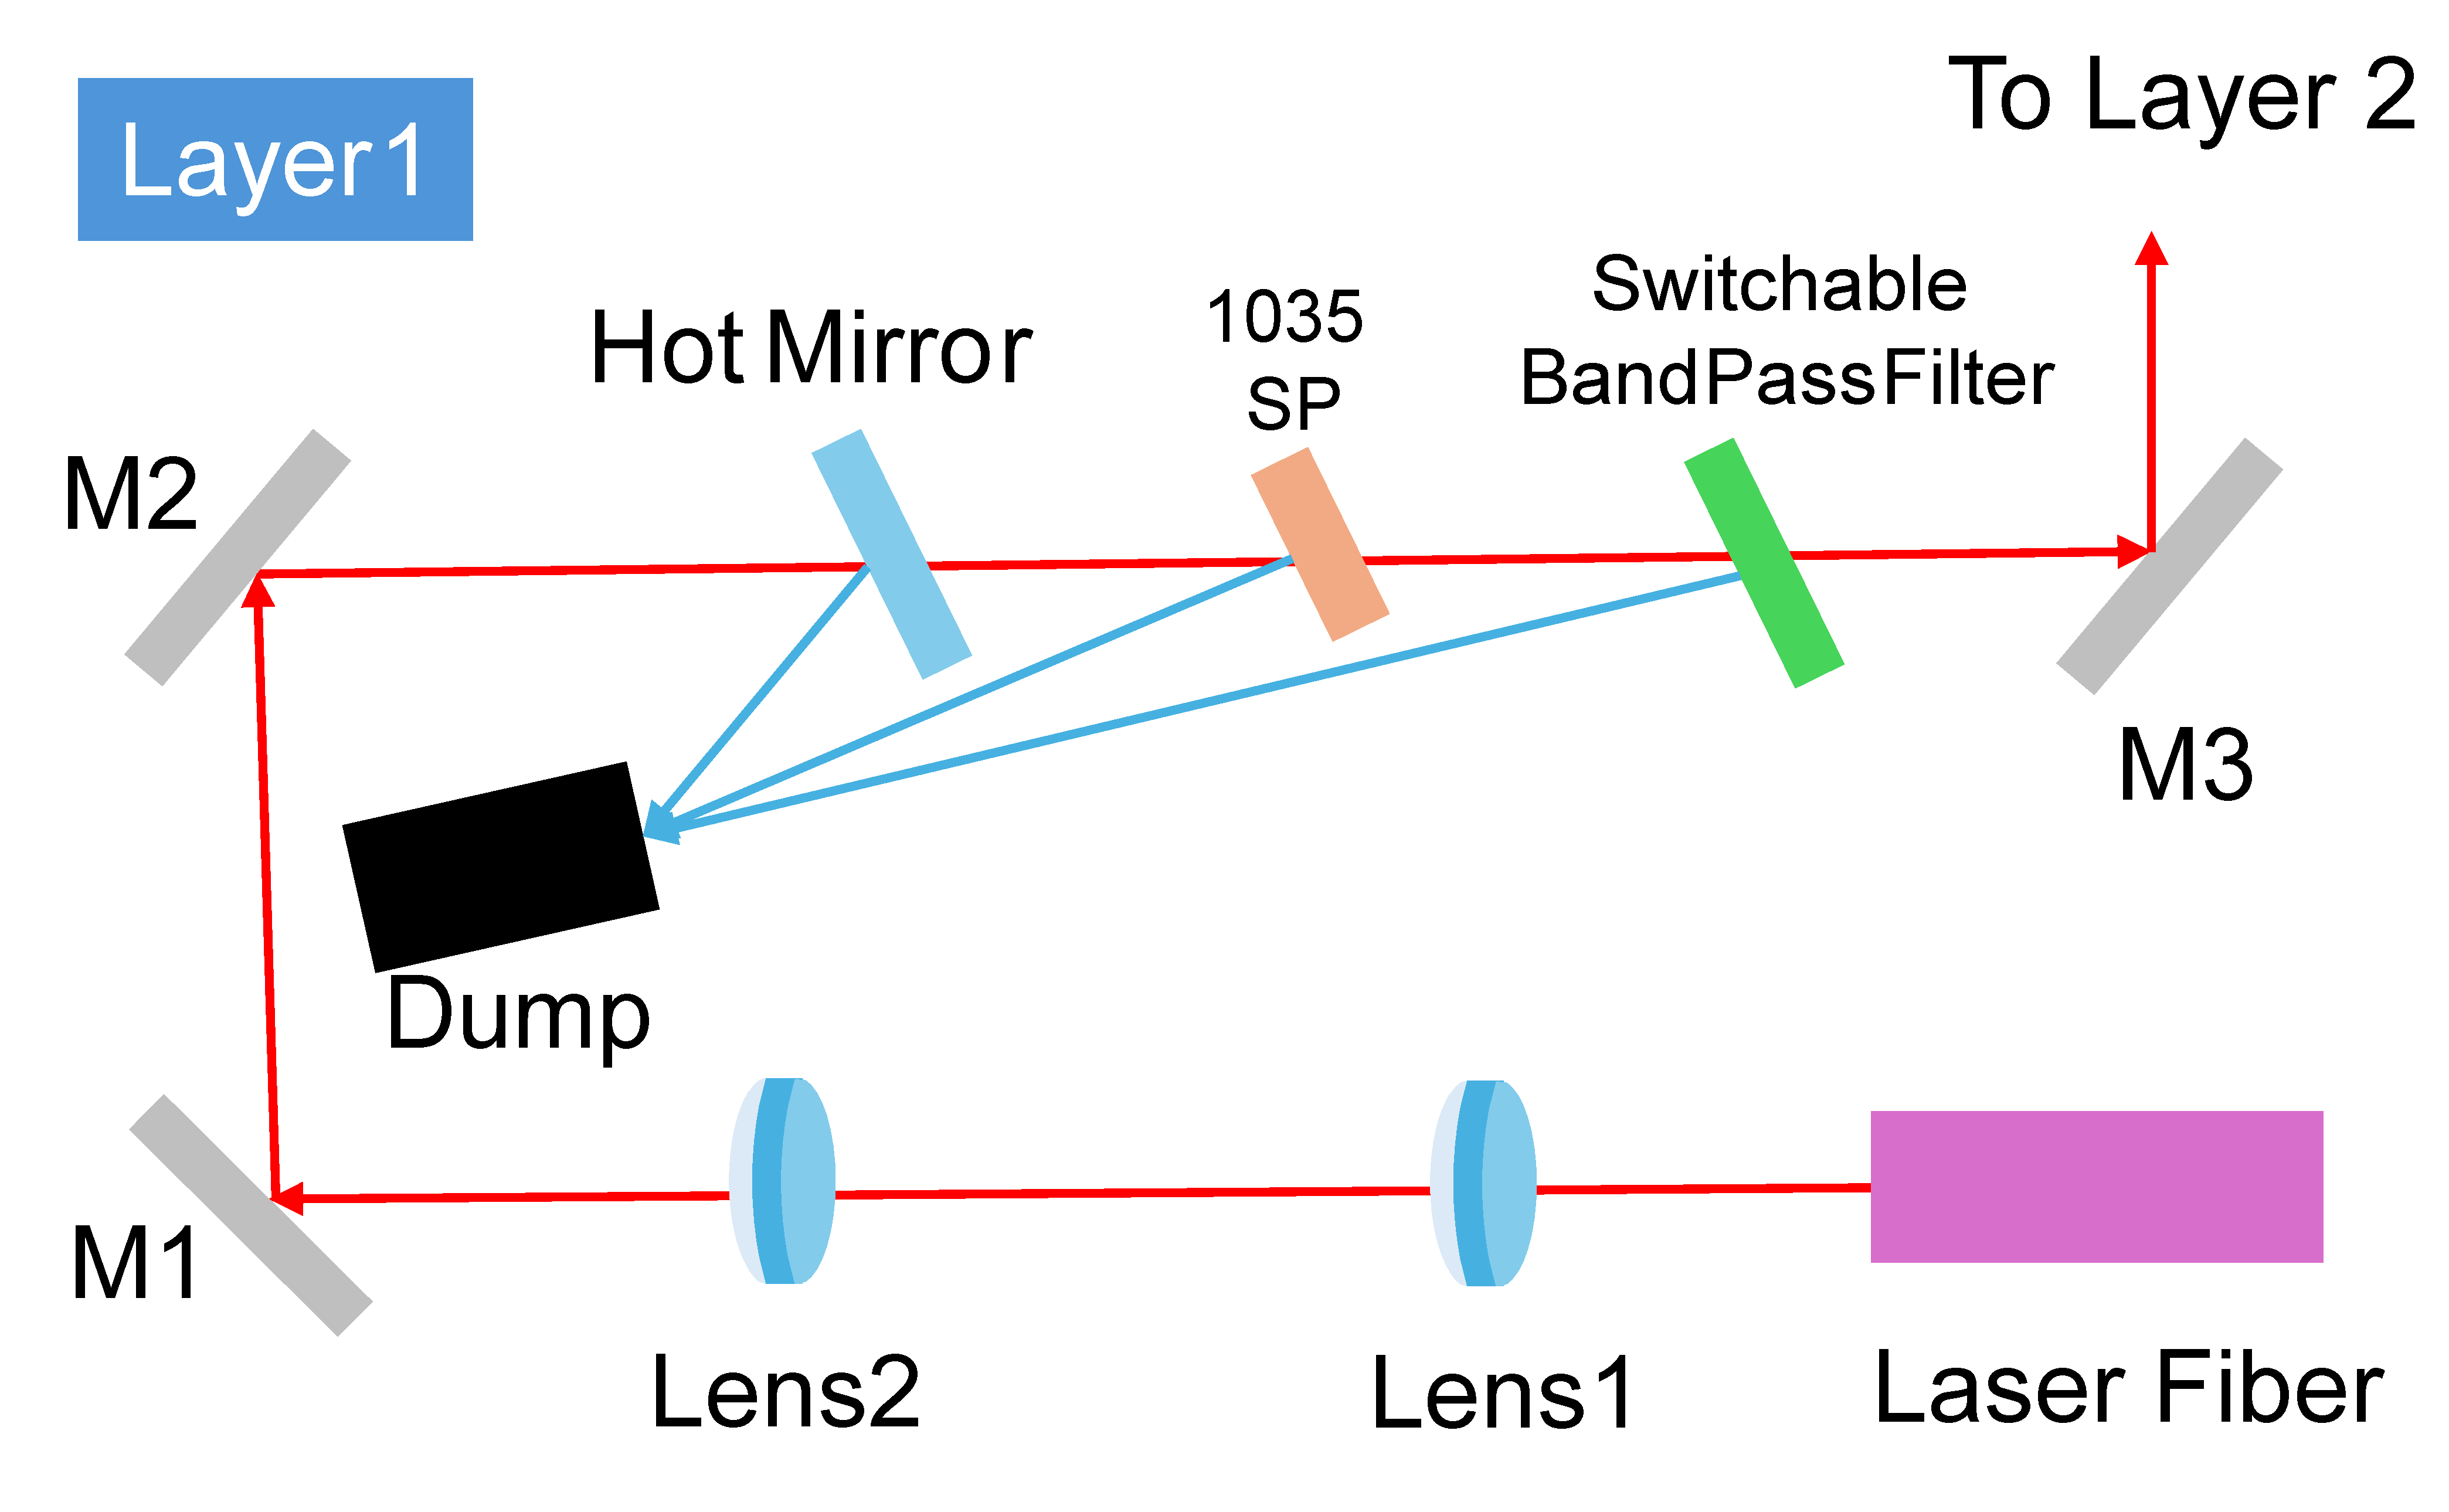
\includegraphics[width=\textwidth]{Fig/FigCon1.pdf}
        \caption{}
        \label{figCon1}
    \end{subfigure}
    \hfill
    \begin{subfigure}[b]{0.53\textwidth}
        \centering
        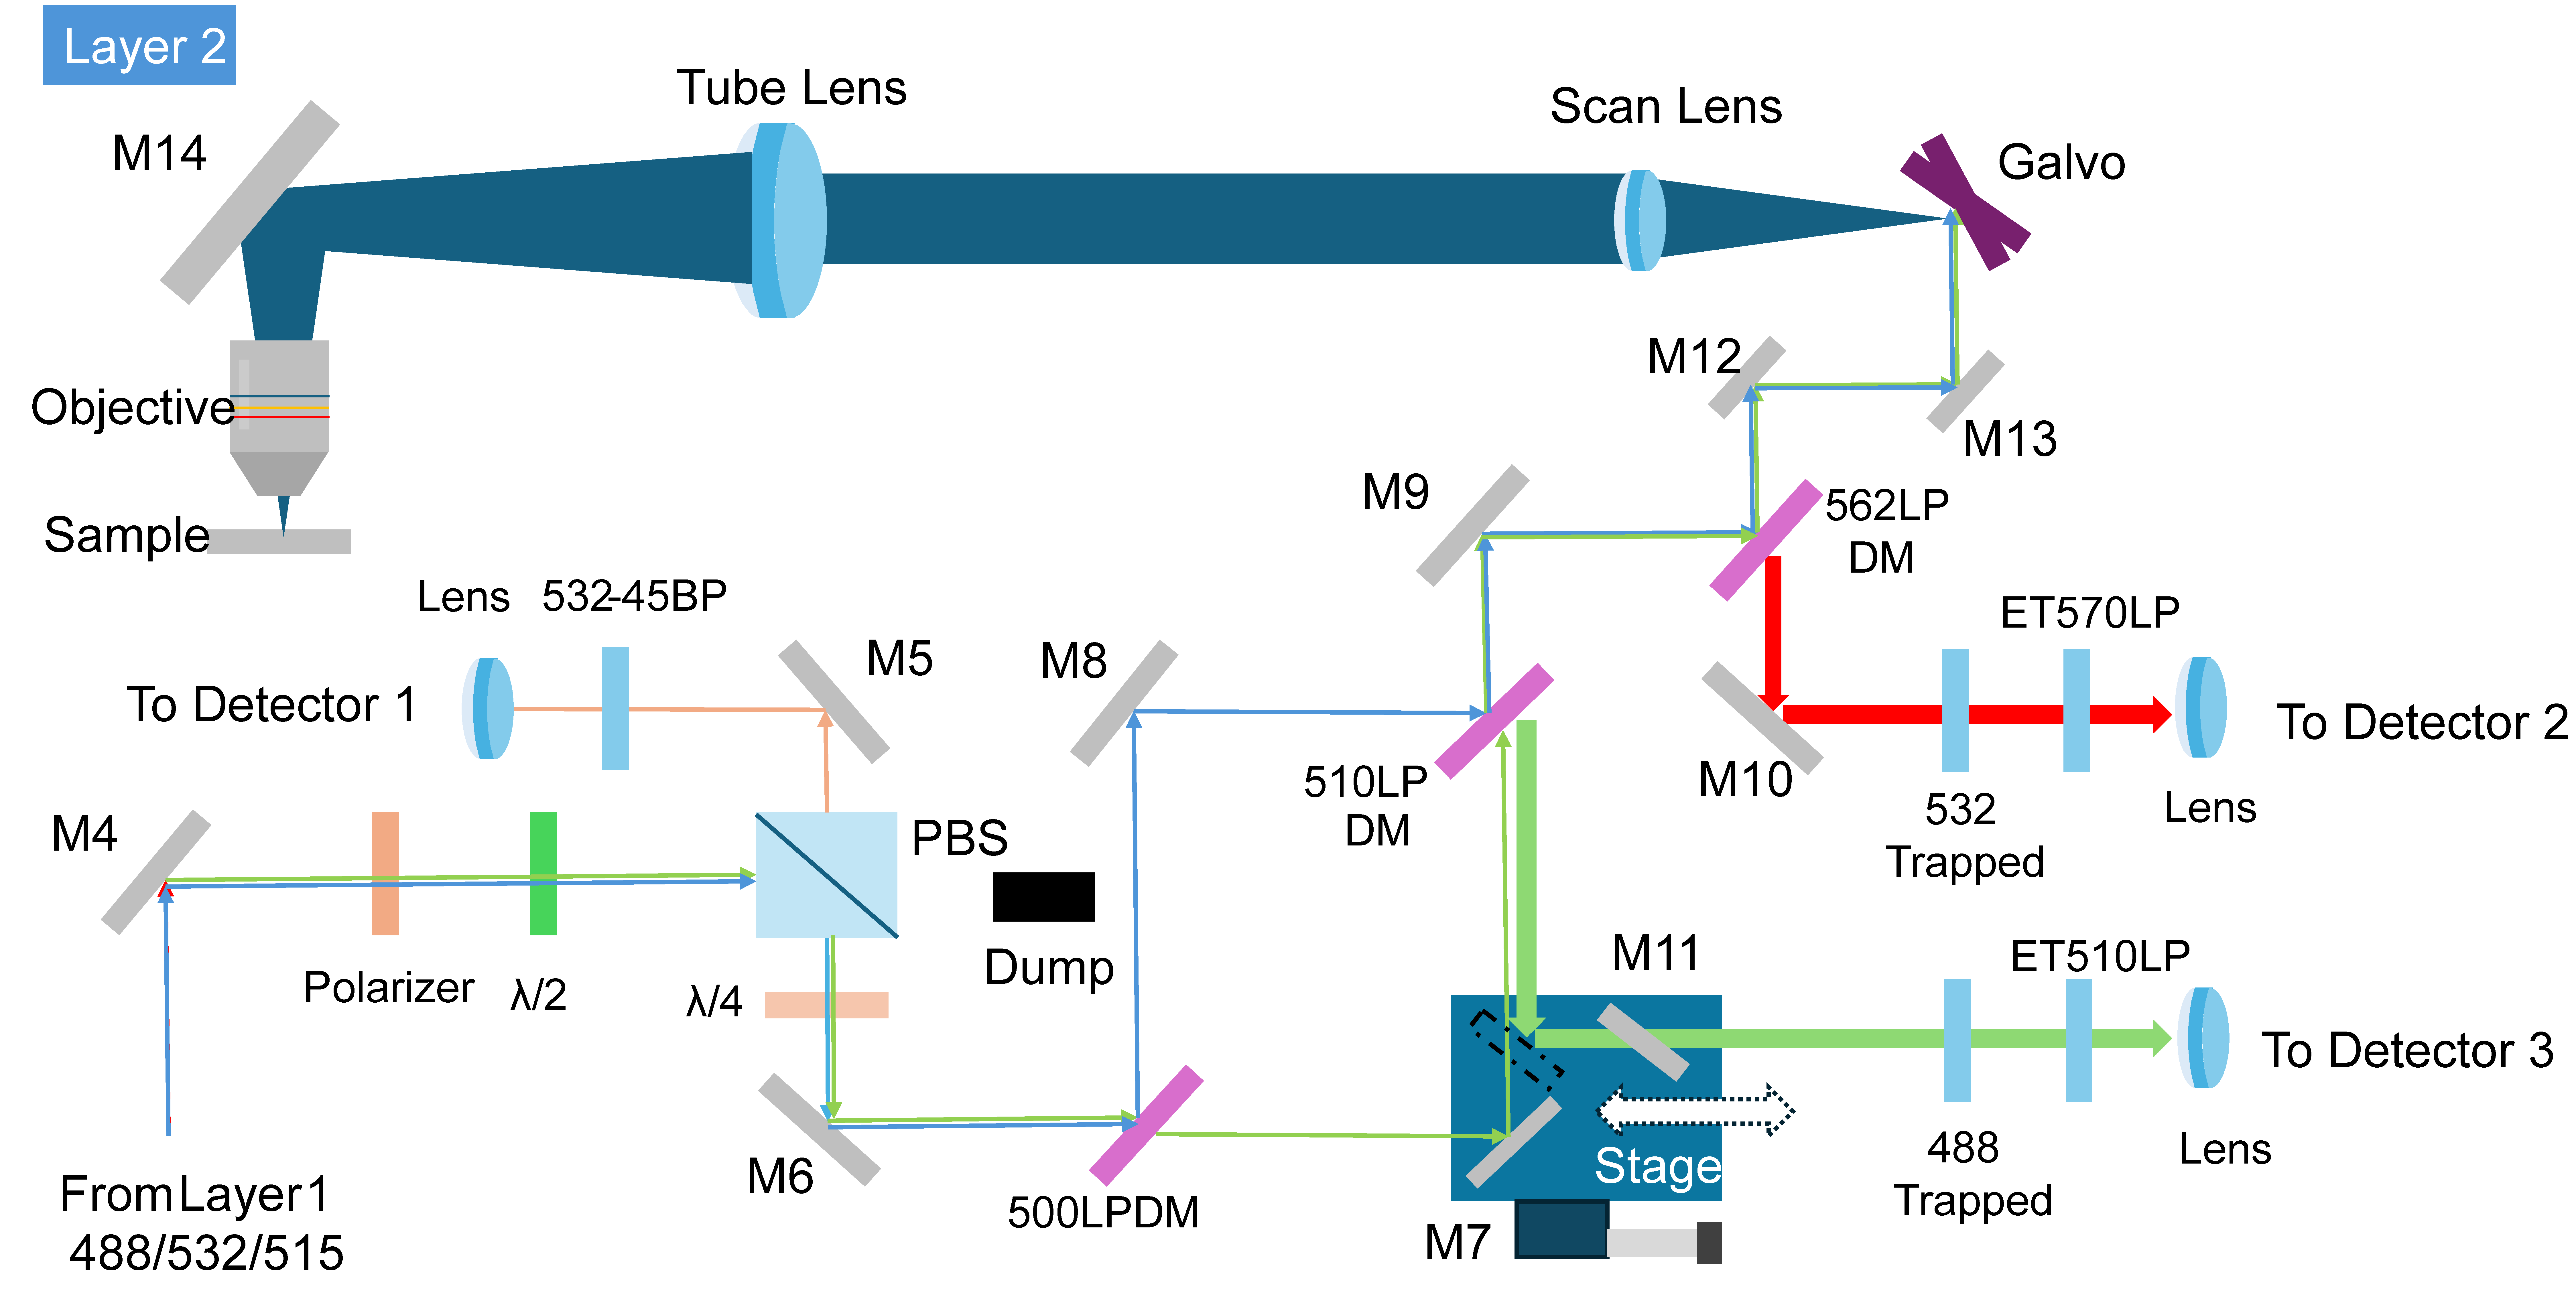
\includegraphics[width=\textwidth]{Fig/FigCon2.pdf}
        \caption{}
        \label{figCon2}
    \end{subfigure}

    \vspace{0.5cm}

    \begin{subfigure}[b]{0.48\textwidth}
        \centering
        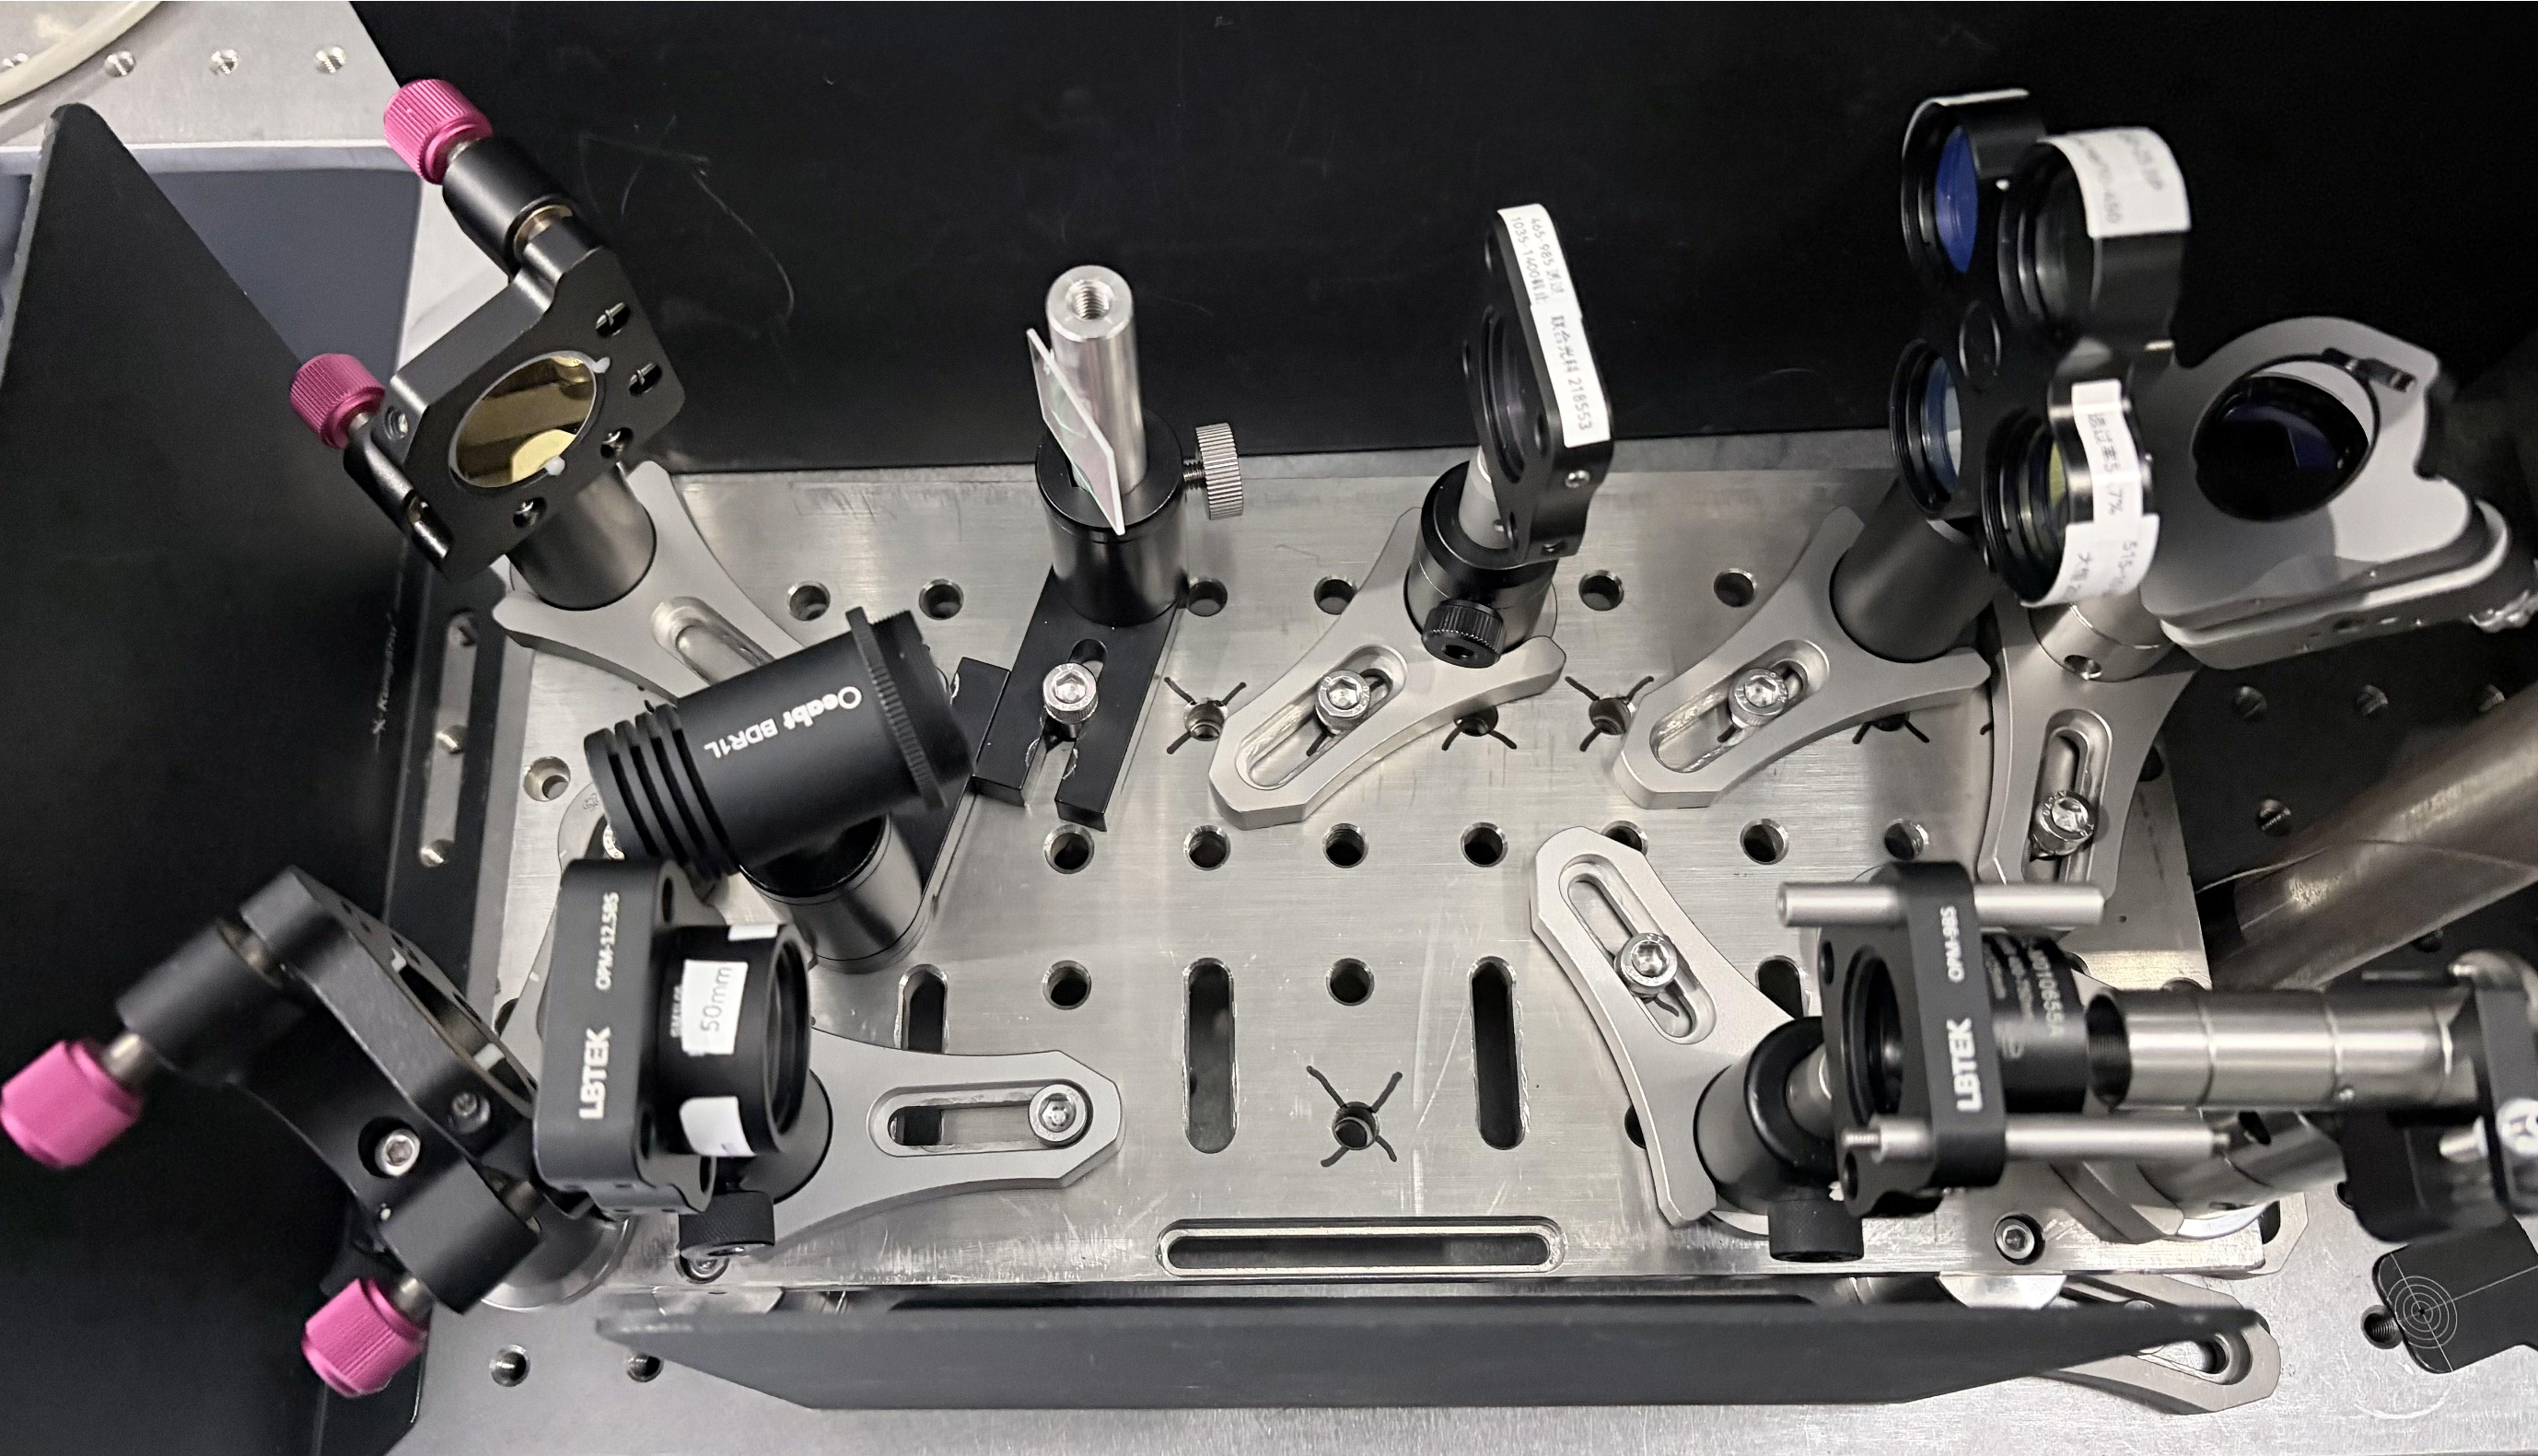
\includegraphics[width=\textwidth]{Fig/FigReal04.pdf}
        \caption{}
        \label{figReal04}
    \end{subfigure}
    \hfill
    \begin{subfigure}[b]{0.48\textwidth}
        \centering
        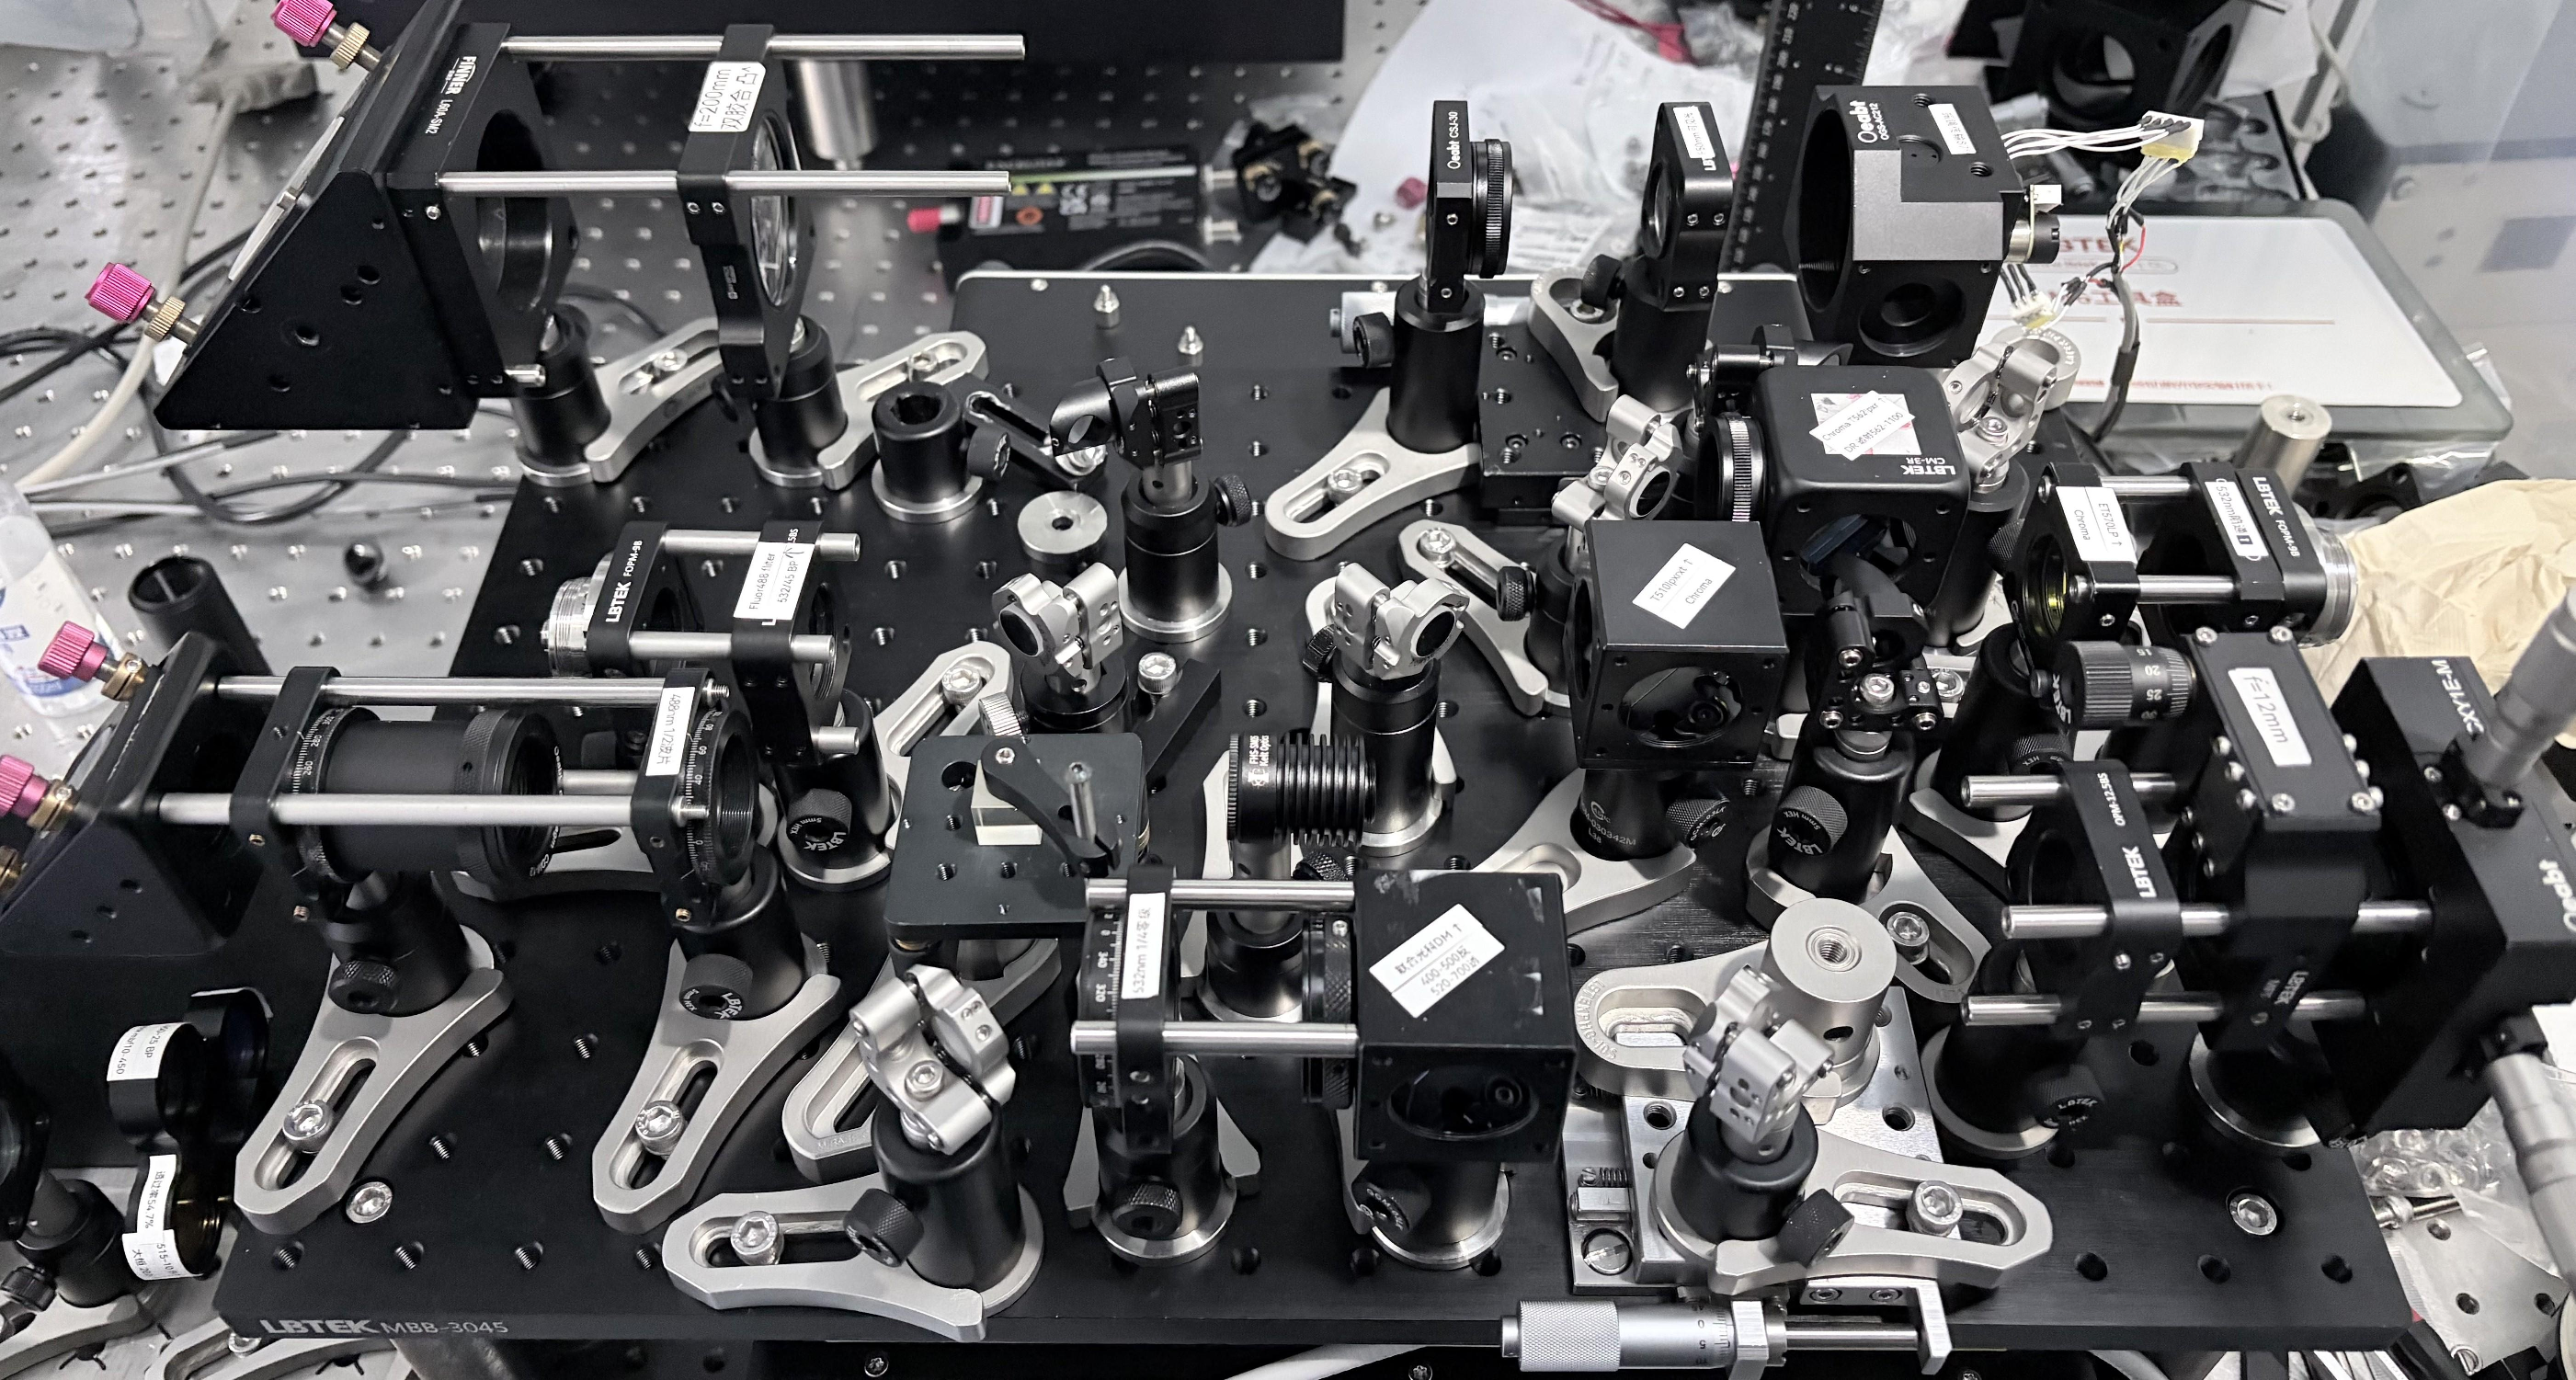
\includegraphics[width=\textwidth]{Fig/FigReal01.pdf}
        \caption{}
        \label{figReal01}
    \end{subfigure}

    \bicaption{多色激发共聚焦系统的原理图与实拍图。(a) 多色共聚焦第一层原理图；(b) 多色共聚焦第二层原理图；(c) 多色共聚焦第一层实拍图；(d) 多色共聚焦第二层实拍图}{Schematics and photographs of the multicolor-excitation confocal system. (a) Schematic of the first layer; (b) schematic of the second layer; (c) photograph of the first layer; (d) photograph of the second layer}
    \label{figConReal}
\end{figure}



\subsection{多色激发与多通道探测方案}

在机械结构实现的基础上，本文进一步构建了一套可实际使用的多色激发荧光共聚焦系统，其原理图与实拍图如图~\ref{figConReal} 所示。该设计以白光 Supercontinuum 超连续谱激光器作为激发源，通过将激发光路和检测光路分开布置，并配置可切换的多组带通滤光片，实现多波长激发条件下的荧光成像。

在激发端，系统配置了 450/30、488/10、515/15 和 532/10 四组带通滤光片(联合光科)，可根据目标荧光探针的激发特性选择任一波段作为激发光。通过这种方式，系统能够在保持主光路不变的情况下灵活实现多波段激发。

在检测端，系统采用了三组长波通二向色镜(Long Pass Dichroic, LP DM)：500LP DM、510LP DM 和 562LP DM(Chroma Inc.)，并结合可切换的千分尺位移台对不同激发波段和发射波段进行分路。以图~\ref{figConReal}(\subref{figCon2}) 为例，绿色细箭头表示 532\,nm 激发光路径，蓝色细箭头表示 488\,nm 激发光路径，红色粗箭头表示 532\,nm 激发下产生的 580\,nm 荧光信号(如 PI 或 Nile Red染料)，绿色粗箭头表示 488\,nm 激发下产生的 530\,nm 荧光信号(如 FITC 或 GFP染料)。通过切换位移台到预设位置，系统可在不同激发/探测模式之间快速切换，同时保留反射信号作为参考通道，以辅助系统对准与结果校验。



\subsection{系统初步性能验证}

\begin{figure}[htbp]
    \centering
    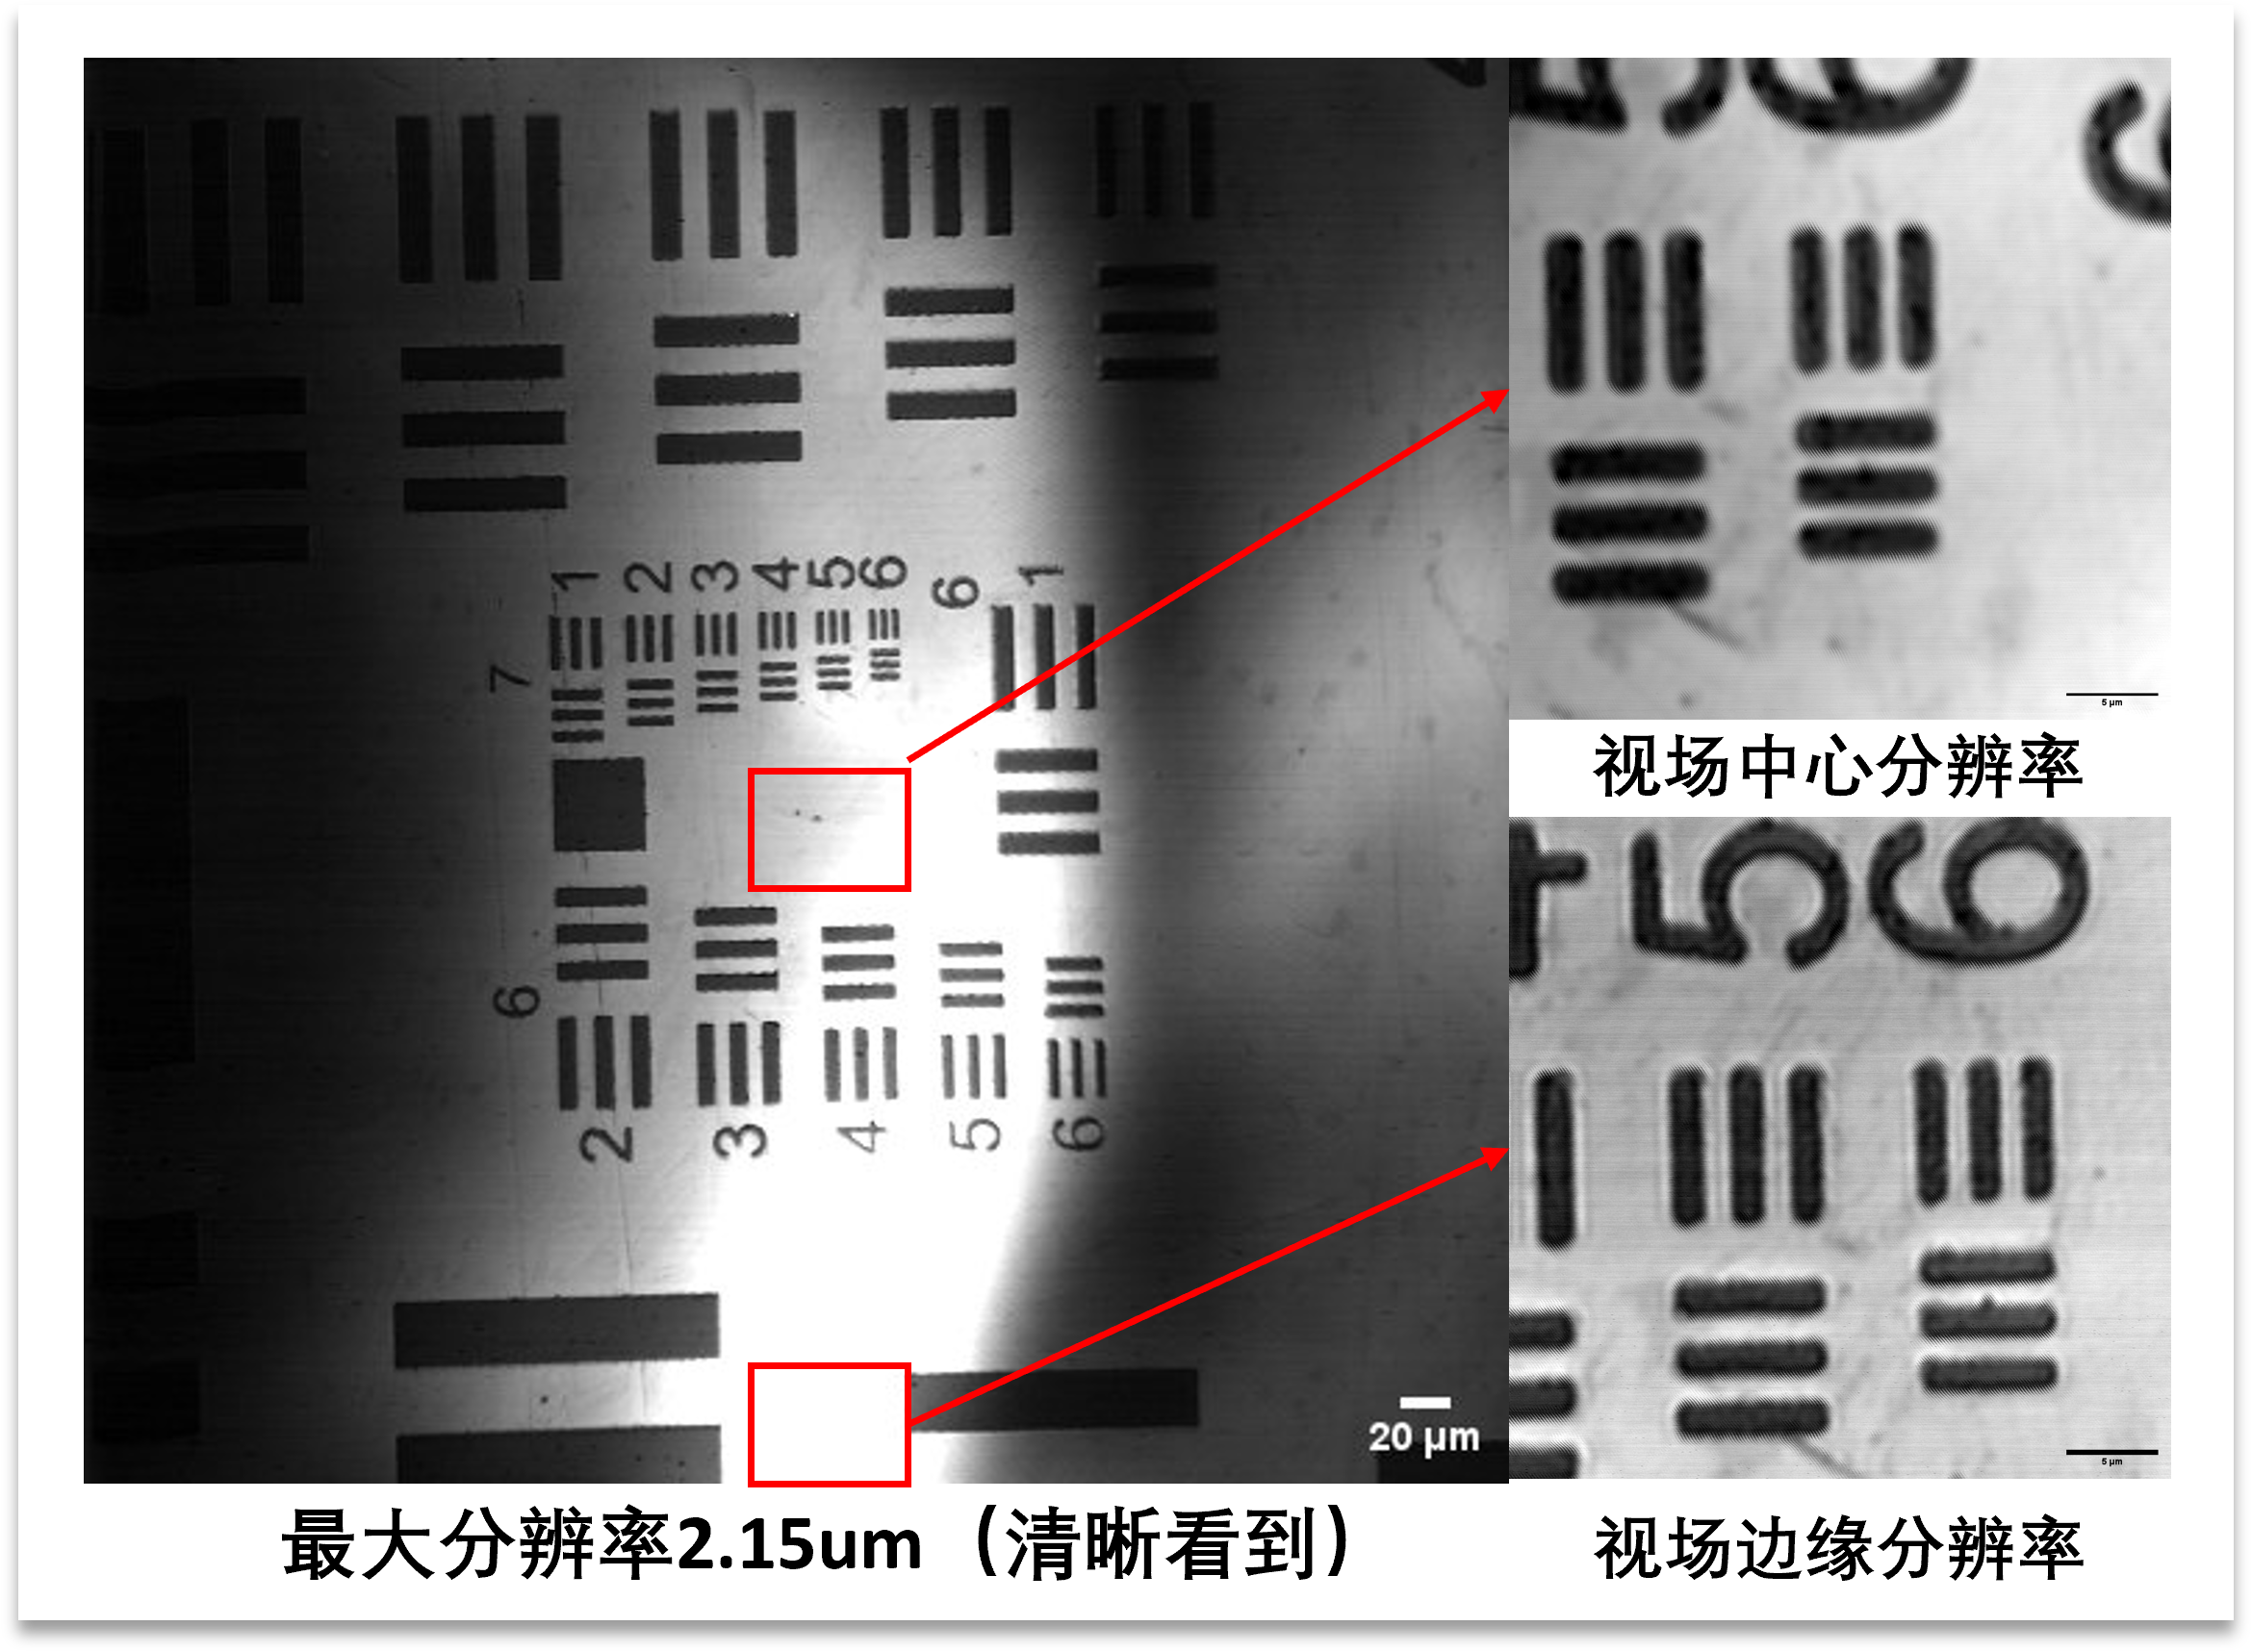
\includegraphics[width=0.55\textwidth]{Fig/Fig38.png}
    \bicaption{使用 USAF 分辨率测试标靶进行分辨率表征}{Resolution characterization using a USAF resolution target}
    \label{fig38}
\end{figure}

在系统光机组装与调试完成后，本文首先对其空间分辨能力进行了初步实验验证。如图~\ref{fig38} 所示，采用标准1951美国空军分辨率测试标靶(1951 USAF resolution test chart, USAF)对系统成像性能进行表征。结果表明，当前系统能够清晰分辨线宽为 2.15\,$\mu$m 的条纹结构，说明系统已经具备较好的显微成像能力和空间分辨能力。

需要指出的是，2.15\,$\mu$m 仅代表 USAF 标靶本身刻线结构中的一个可分辨尺度，并不能直接等同于本系统的真实衍射极限。为了进一步定量测量系统点扩散函数并获得更准确的横向与轴向分辨率参数，后续还需采用尺寸远小于工作波长的荧光微球进行 PSF 标定与分析。因此，本节中的 USAF 标靶测试更适合作为系统已具备基本成像能力的初步验证，而更精确的系统分辨率评估将在后续实验中进一步开展。

总体而言，本章围绕白光超连续谱与多色激发共聚焦显微系统的方案设计、机械实现和初步性能验证，完成了从概念构型到实体搭建的关键过渡。后续工作可进一步结合标准荧光样品、荧光微球和典型生物样本，对系统的分辨率、通道串扰、激发/探测切换稳定性以及多色成像一致性开展更系统的定量表征，从而为该平台在多通道荧光成像、反射成像与寿命成像中的进一步应用奠定基础。



% \subsection{图像扫描显微镜(ISM)的提出与发展}

% 图像扫描显微镜(Image Scanning Microscopy, ISM)可以看作是在传统共聚焦显微镜基础上发展起来的一类高效成像方法，其目标是在尽量保持较高光子利用率的前提下，进一步提升空间分辨率。该技术的发展与共聚焦显微镜的局限密切相关:经典共聚焦通过缩小小孔能够获得更好的分辨率与切片能力，但代价是信号大幅损失；若采用较大的小孔，则虽能提高信号收集效率，却会削弱共焦优势。ISM 的提出正是为了缓解这一对矛盾。

% 从技术演进角度看，早期共聚焦显微镜通常采用单点探测器(如光电倍增管)配合小孔进行信号采集，其探测信息仅表现为某一扫描位置上的总光强值，无法进一步利用焦斑内部的空间分布信息。随着面阵探测器、小型高灵敏探测阵列以及高速数据采集技术的发展，研究人员开始考虑在扫描过程中保留每一个扫描点对应的局部荧光图样，而不仅是记录其积分强度。基于这一思想，图像扫描显微镜逐渐形成并发展起来。它将传统``点探测''扩展为``阵列探测''，从而为后续的像素重定位(pixel reassignment)、图像融合与分辨率提升提供了基础。

% 随后，ISM 与计算成像思想进一步结合，形成了多种实现形式。例如，通过单光子雪崩二极管阵列(SPAD array)、sCMOS 或 CCD 探测器对扫描点的荧光分布进行采集，再结合像素重分配算法，可在不显著降低信号的情况下实现比传统共聚焦更高的分辨率。同时，ISM 还可与荧光寿命探测、时间门控、光子计数及自适应光学等方法结合，扩展其在活体成像、高速成像和弱信号探测中的应用能力。近年来，随着高灵敏度探测阵列和高速并行读出电路的发展，ISM 已成为连接传统共聚焦与计算超分辨成像的重要技术路线之一。

% \subsection{ISM 的基本原理}

% ISM 的核心思想是在激光逐点扫描样品的过程中，不再使用单一探测器记录每个扫描位置处的总荧光强度，而是利用一个小型探测器阵列记录扫描焦点对应的局部像分布。也就是说，对于样品上的每一个扫描位置，系统得到的不是一个标量信号，而是一组来自不同探测单元的强度信息。由于阵列中各探测单元相对于光轴存在不同空间偏移，因此它们所接收到的信号对应于样品信息的不同采样视角。

% 从成像模型上看，传统共聚焦显微镜的有效点扩散函数可表示为激发点扩散函数与探测点扩散函数的乘积；在 ISM 中，阵列上每个探测单元都对应一个略有偏移的探测点扩散函数，因此每个通道实际上都形成一幅具有轻微位移的信息子图像。若直接将这些子图像简单叠加，虽然可以提高信号，但无法充分发挥阵列探测带来的分辨优势。为此，ISM 采用像素重分配方法，将每个探测通道对应的信号按照其空间偏移重新映射到更接近真实发光位置的坐标上，再对所有通道的重分配结果进行累加。由于每个通道都贡献了更准确的空间定位信息，最终重建得到的图像在保持较高信噪比的同时，其点扩散函数会变窄，从而实现优于传统共聚焦的分辨率。

% 在理想情况下，像素重分配后的 ISM 图像横向分辨率相较于宽场成像可获得更明显提升，同时又避免了传统共聚焦中因小孔过小而导致的严重光子损失。其本质原因在于:传统小孔会直接丢弃部分离轴信号，而 ISM 则尝试将这些本可被舍弃的光子重新利用，并借助探测阵列的空间信息将其``放回''更合理的位置。因此，ISM 可以理解为一种兼顾高光子效率与高分辨率的``信息回收型共聚焦成像''方法。

% \subsection{像素重分配机制}

% 像素重分配(Pixel Reassignment)是 ISM 最具代表性的图像重建方法之一，也是其分辨率提升的关键。对于阵列探测器中的某一离轴探测单元，其记录到的局部图像并不与真实发光位置完全重合，而是相对中心通道发生了偏移。这个偏移来源于激发焦斑与探测通道位置共同决定的系统响应。理论分析表明，对于荧光发射过程，在激发与探测点扩散函数形状近似相同的条件下，各探测通道信息子图像的最佳重定位量通常接近其探测单元位移的一半。因此，可以将阵列上每个通道采集的数据沿适当方向移动一定距离，再将所有重分配后的子图像进行求和，从而获得分辨率更高的最终图像。

% 该过程之所以有效，是因为它并不是简单地缩小光斑，而是利用多个探测通道对同一发光事件的冗余观测信息，提高了信号定位精度。相比于直接减小共焦小孔，像素重分配并未显著牺牲总光子数，因此在弱荧光样品成像中具有更强实用性。对于噪声受限系统，这种``先采集、后重构''的策略尤其有利，因为它避免了在硬件层面主动丢失信号。

% 在工程实现上，像素重分配可以通过理论模型确定重定位参数，也可以通过实验标定方式得到更加精确的偏移量。例如，利用纳米荧光珠测量系统点扩散函数后，对各通道响应中心进行拟合，即可建立探测单元与图像重定位之间的映射关系。若系统存在像差、放大率误差或探测阵列安装偏差，实验标定方法通常能够获得比理想模型更准确的重建结果。

% \subsection{ISM 与传统共聚焦显微镜的比较}

% 与传统 LSCM 相比，ISM 在成像思想和信号利用方式上均有所扩展。传统共聚焦的主要手段是通过缩小小孔来压制离焦背景，其性能提升依赖于硬件层面的空间截断；而 ISM 则更强调对探测信息的充分利用，通过阵列探测与计算重构，在保留较多光子的同时实现分辨率增强。两者都属于扫描显微成像范畴，也都具备较好的光学切片能力，但 ISM 在光子利用效率和后端重建灵活性方面具有明显优势。

% 从分辨率角度看，传统共聚焦的提升主要来自激发与探测点扩散函数的乘积效应；ISM 则进一步借助多通道空间信息和像素重分配机制缩窄有效点扩散函数。对于信号较弱、样品易漂白或需要高速采集的应用场景，ISM 往往比``小孔极限''下的共聚焦更具应用价值。另一方面，ISM 也引入了更高的数据量和更复杂的计算需求，对探测器阵列性能、同步采集精度以及重建算法稳定性提出了更高要求。

% \subsection{共聚焦与 ISM 在超分辨发展中的意义}

% 从显微成像技术的发展脉络来看，共聚焦显微镜是现代荧光显微技术中承上启下的重要平台。一方面，它相较于宽场荧光显著提高了图像对比度、轴向分辨率和三维层析能力；另一方面，它又为后续诸多超分辨与计算成像方法提供了基础架构。许多高分辨成像方法都继承了共聚焦的逐点扫描思想，并在激发调控、探测方式或信号重构策略上加以拓展。

% ISM 正是在这一背景下发展起来的代表性技术。它并未像 STED 那样通过非线性光学效应直接压缩发光体积，也不同于单分子定位显微术通过时域稀疏激活实现分辨率突破，而是通过改进探测策略与重建算法，在传统扫描显微框架内实现性能增强。因此，ISM 通常被视为一种介于经典共聚焦与严格意义上的超分辨显微技术之间的方法:它能够在较低光损伤和较高光子效率条件下取得优于传统共聚焦的成像效果，并为后续更高阶的计算超分辨方法提供了良好的技术基础。
